\documentclass[a4paper,11pt]{article}
\usepackage{amsfonts}
\usepackage{amssymb}
\usepackage{amsmath}
\usepackage{euscript}
\usepackage{boxedminipage}
\usepackage{lscape}
\usepackage{minitoc}
\usepackage{epsfig,psfrag,graphicx,verbatim}
\usepackage{url,natbib}
\usepackage{booktabs, longtable}
\vfuzz2pt % Don't report over-full v-boxes if over-edge is small
\hfuzz2pt % Don't report over-full h-boxes if over-edge is small
\setlength{\oddsidemargin}{0cm}
\setlength{\evensidemargin}{0cm}
\setlength{\textwidth}{16cm}
\setlength{\textheight}{23cm}
\title{Eurace}
\author{to add}
\date{\today}
\begin{document}
\maketitle
\tableofcontents
\clearpage
\section{Eurace FLAME Implementation}
\subsection{Firm}

\subsubsection{Memory}

Table \ref{Table: Firm Memory}.
\begin{center}
\begin{longtable}[H!]{ll}
\caption{{\bfseries List of memory variables.}}
\label{Table: Firm Memory}\\
\toprule 
 Name & Description \\
\midrule
\endfirsthead
\multicolumn{2}{c}%
{{\bfseries \tablename\ \thetable{} -- continued from previous page}} \\
\toprule
 Name & Description \\
\midrule
\endhead
\multicolumn{2}{r}{{\emph{Continued on next page}}} \\
\endfoot
\bottomrule
\endlastfoot
\url{int} \url{id} & \parbox{10cm}{Agent ID.} \\
\url{int} \url{region_id} & \parbox{10cm}{Region ID to which the agent is associated.} \\
\url{int} \url{gov_id} & \parbox{10cm}{Government  to which the agent is associated.} \\
\url{int} \url{day_of_month_to_act} & \parbox{10cm}{Activation day.} \\
\url{int} \url{last_day_of_month_to_act} & \parbox{10cm}{One day before the activation day.} \\
\url{double} \url{payment_account} & \parbox{10cm}{Current account value.} \\
\url{int} \url{bank_id} & \parbox{10cm}{Bank ID at which the agent maintains its payment account.} \\
\url{int} \url{partition_id} & \parbox{10cm}{Partition ID used for parallelization.} \\
\url{double} \url{cpi} & \parbox{10cm}{This is the CPI in firm memory, used in the evaluation of the inventory stock.} \\
\url{double} \url{mean_wage} & \parbox{10cm}{Average wage paid by a firm} \\
\url{double} \url{needed_capital_stock} & \parbox{10cm}{The overall capital stock a firm wants to have} \\
\url{double} \url{actual_cap_price} & \parbox{10cm}{Price of the latest capital good} \\
\url{double} \url{mean_specific_skills} & \parbox{10cm}{Average specific skills of the workforce} \\
\url{double} \url{planned_production_quantity} & \parbox{10cm}{Planned production quantity, has a value on production day, but is reset on other days.} \\
\url{double} \url{production_quantity} & \parbox{10cm}{Actual production quantity, has a value on production day, but is reset on other days.} \\
\url{double} \url{planned_output} & \parbox{10cm}{Planned output is the same as planned production quantity, but retains its value during the month.} \\
\url{double} \url{output} & \parbox{10cm}{Actual output is the same as production quantity, but retains its value during the month.} \\
\url{double} \url{unit_costs} & \parbox{10cm}{Cost per unit of the consumption good} \\
\url{double} \url{total_supply} & \parbox{10cm}{The sum of local inventory and produced output gives the total supplied quantity} \\
\url{double} \url{production_costs} & \parbox{10cm}{Actual production costs, labor and capital} \\
\url{double} \url{revenue_per_day} & \parbox{10cm}{Daily revenue} \\
\url{estimators_linear_regression_array} \url{linear_regression_estimators} & \parbox{10cm}{Holds the estimators for the linear regression model} \\
\url{double} \url{technological_frontier} & \parbox{10cm}{Best available technology in the economy} \\
\url{double} \url{cum_revenue} & \parbox{10cm}{Monthly revenue} \\
\url{double} \url{out_of_stock_costs} & \parbox{10cm}{} \\
\url{sales_statistics_array} \url{malls_sales_statistics} & \parbox{10cm}{Sales of the last ten months} \\
\url{double} \url{quality} & \parbox{10cm}{Quality of the consumption good} \\
\url{double} \url{price} & \parbox{10cm}{Price of the consumption good} \\
\url{double} \url{price_last_month} & \parbox{10cm}{Price of the consumption good in the last month} \\
\url{int} \url{decil_production_rule} & \parbox{10cm}{Actual output is the same as production quantity, but retains its value during the month.} \\
\url{double} \url{demand_capital_stock} & \parbox{10cm}{Demand for capital goods} \\
\url{double} \url{planned_production_costs} & \parbox{10cm}{ Planned production costs} \\
\url{double} \url{adaption_production_volume_due_to_insufficient_finances} & \parbox{10cm}{Percentage of production by which the quantity is reduced} \\
\url{double} \url{fraction_reserved_for_delayed_payments} & \parbox{10cm}{} \\
\url{sold_quantities_per_mall_array} \url{sold_quantities} & \parbox{10cm}{Sold quantities in the different malls} \\
\url{double} \url{total_sold_quantity} & \parbox{10cm}{Daily sum of sold quantities in all malls. The sold quantity of one firm in all malls.} \\
\url{double} \url{cum_total_sold_quantity} & \parbox{10cm}{Monthly sum of sold quantities in all malls. The monthly sold quantity of one firm in all malls.} \\
\url{double} \url{sold_quantity_in_calendar_month} & \parbox{10cm}{Monthly sum of sold quantities in all malls. The quantity sold in one calendar month.} \\
\url{delivery_volume_per_mall_array} \url{delivery_volume} & \parbox{10cm}{Delivery volume for each mall} \\
\url{delivery_volume_per_mall_array} \url{planned_delivery_volume} & \parbox{10cm}{Planned delivery volume for each  mall} \\
\url{mall_info_array} \url{current_mall_stocks} & \parbox{10cm}{Current stock in each mall} \\
\url{double_array} \url{last_planned_production_quantities} & \parbox{10cm}{Array of the planned production quantities in the past} \\
\url{double} \url{total_external_financing_obtained} & \parbox{10cm}{} \\
\url{double} \url{capital_costs} & \parbox{10cm}{} \\
\url{double} \url{labour_costs} & \parbox{10cm}{} \\
\url{financing_capital_array} \url{capital_financing} & \parbox{10cm}{} \\
\url{double} \url{financial_resources_for_production} & \parbox{10cm}{} \\
\url{double} \url{planned_value_capital_stock} & \parbox{10cm}{} \\
\url{double} \url{total_units_local_inventory} & \parbox{10cm}{} \\
\url{double} \url{calc_capital_costs} & \parbox{10cm}{Calculative capital costs} \\
\url{double} \url{calc_production_costs} & \parbox{10cm}{Calculative production costs} \\
\url{double} \url{firm_productivity} & \parbox{10cm}{min of technology and mean\_specific\_skills} \\
\url{double} \url{firm_productivity_last_year} & \parbox{10cm}{} \\
\url{double} \url{firm_productivity_progress} & \parbox{10cm}{} \\
\url{potential_lender_array} \url{set_of_lenders} & \parbox{10cm}{Array of structs (potential lender) holding names of (found) active banks.} \\
\url{int} \url{number_of_banks_asked} & \parbox{10cm}{Number of banks where the firm has asked for loans.} \\
\url{double} \url{ebit} & \parbox{10cm}{Earnings-before-interest-and-taxes: total revenue - sales\_costs} \\
\url{double} \url{earnings} & \parbox{10cm}{Earnings after interest payments (= ebit - interest)} \\
\url{double} \url{tax_rate_corporate} & \parbox{10cm}{Tax rate on corporate profits (kept in memory)} \\
\url{double} \url{tax_rate_vat} & \parbox{10cm}{VAT tax rate} \\
\url{double} \url{tax_payment} & \parbox{10cm}{Tax payment over earnings after interest payments (tax\_corporate*earnings)} \\
\url{double} \url{net_earnings} & \parbox{10cm}{Net earnings after tax payments (= ebit - interest - tax)} \\
\url{double} \url{previous_net_earnings} & \parbox{10cm}{Net earnings from previous production period} \\
\url{double} \url{total_interest_payment} & \parbox{10cm}{Total interest payments on outstanding debts} \\
\url{double} \url{total_debt_installment_payment} & \parbox{10cm}{Total debt installment payments on outstanding debts} \\
\url{double} \url{total_dividend_payment} & \parbox{10cm}{Total dividend payment} \\
\url{double} \url{current_share_price} & \parbox{10cm}{Current share price on the market} \\
\url{double} \url{previous_dividend_per_share} & \parbox{10cm}{Dividend-per-share ratio (previous production cycle)} \\
\url{double} \url{current_dividend_per_share} & \parbox{10cm}{Dividend-per-share ratio} \\
\url{double} \url{previous_earnings_per_share} & \parbox{10cm}{Earnings-per-Share ratio (previous production cycle)} \\
\url{double} \url{current_earnings_per_share} & \parbox{10cm}{Earnings-per-Share ratio} \\
\url{double} \url{previous_dividend_per_earnings} & \parbox{10cm}{Dividend-to-Earnings ratio (previous production cycle)} \\
\url{double} \url{current_dividend_per_earnings} & \parbox{10cm}{Dividend-to-Earnings ratio} \\
\url{double} \url{debt_earnings_ratio} & \parbox{10cm}{Debt-to-Earnings ratio} \\
\url{double} \url{debt_equity_ratio} & \parbox{10cm}{Debt-to-Equity ratio} \\
\url{double} \url{price_earnings_ratio} & \parbox{10cm}{Price-to-Earnings ratio} \\
\url{double} \url{retained_earnings_ratio} & \parbox{10cm}{Retained earnings-to-Earnings ratio} \\
\url{double} \url{earnings_per_share_ratio_growth} & \parbox{10cm}{Target growth of the Earnings-per-Share ratio} \\
\url{double} \url{critical_price_earnings_ratio} & \parbox{10cm}{Critical (target) value for the Price-Earnings ratio (can be set by the firm)} \\
\url{double} \url{critical_earnings_per_share_ratio} & \parbox{10cm}{Critical (target) value for the Earnings-per-Share ratio (derived from the growth level)} \\
\url{debt_item_array} \url{loans} & \parbox{10cm}{Array of structs holding all loans of the firm} \\
\url{double} \url{total_debt} & \parbox{10cm}{Total value of all loans outstanding} \\
\url{double} \url{total_value_local_inventory} & \parbox{10cm}{Total value of all local inventory stocks held at malls} \\
\url{double} \url{total_units_capital_stock} & \parbox{10cm}{Units of capital stock} \\
\url{double} \url{total_value_capital_stock} & \parbox{10cm}{Value of the capital stock} \\
\url{double} \url{total_capital_depreciation_value} & \parbox{10cm}{Sum over all units of capital of the depreciation value} \\
\url{double} \url{total_capital_depreciation_units} & \parbox{10cm}{Sum over all units of capital of the depreciation in units} \\
\url{double} \url{total_assets} & \parbox{10cm}{Value of total assets} \\
\url{double} \url{equity} & \parbox{10cm}{equity = total assets - total liabilities} \\
\url{double} \url{production_liquidity_needs} & \parbox{10cm}{Production liquidity needs are production costs (labour costs and investments)} \\
\url{double} \url{financial_liquidity_needs} & \parbox{10cm}{Financial liquidity needs are prior financial commitments (interests, installments, taxes)} \\
\url{double} \url{total_financial_needs} & \parbox{10cm}{Total financial needs = Production liquidity needs + Financial liquidity needs + dividends} \\
\url{double} \url{external_financial_needs} & \parbox{10cm}{External financing} \\
\url{double} \url{earnings_per_share} & \parbox{10cm}{} \\
\url{double} \url{total_payments} & \parbox{10cm}{} \\
\url{int} \url{previous_shares_outstanding} & \parbox{10cm}{} \\
\url{double} \url{total_income} & \parbox{10cm}{Total monthly income (revenues, new bank loans, new share issues). Used for the balance sheet accounting.} \\
\url{double} \url{total_liabilities} & \parbox{10cm}{} \\
\url{double} \url{total_expenses} & \parbox{10cm}{} \\
\url{double} \url{earnings_payout} & \parbox{10cm}{} \\
\url{int} \url{current_shares_outstanding} & \parbox{10cm}{} \\
\url{Stock} \url{stock} & \parbox{10cm}{} \\
\url{employee_array} \url{employees} & \parbox{10cm}{Used to store the data-type Employee} \\
\url{double} \url{wage_offer} & \parbox{10cm}{The basic wage offer paid per unit of specific skills} \\
\url{double} \url{technology} & \parbox{10cm}{Average technology/productivity of the capital} \\
\url{int} \url{no_employees} & \parbox{10cm}{Number of employees} \\
\url{int} \url{no_employees_skill_1} & \parbox{10cm}{Number of employees with general skills 1} \\
\url{int} \url{no_employees_skill_2} & \parbox{10cm}{Number of employees with general skills 2} \\
\url{int} \url{no_employees_skill_3} & \parbox{10cm}{Number of employees with general skills 3} \\
\url{int} \url{no_employees_skill_4} & \parbox{10cm}{Number of employees with general skills 4} \\
\url{int} \url{no_employees_skill_5} & \parbox{10cm}{Number of employees with general skills 5} \\
\url{int} \url{vacancies} & \parbox{10cm}{Number of vacancies} \\
\url{double} \url{average_g_skill} & \parbox{10cm}{Average general skills of the workforce} \\
\url{double} \url{average_s_skill_of_1} & \parbox{10cm}{Average specific skills of employees with general skills 1} \\
\url{double} \url{average_s_skill_of_2} & \parbox{10cm}{Average specific skills of employees with general skills 2} \\
\url{double} \url{average_s_skill_of_3} & \parbox{10cm}{Average specific skills of employees with general skills 3} \\
\url{double} \url{average_s_skill_of_4} & \parbox{10cm}{Average specific skills of employees with general skills 4} \\
\url{double} \url{average_s_skill_of_5} & \parbox{10cm}{Average specific skills of employees with general skills 5} \\
\url{double} \url{wage_offer_for_skill_1} & \parbox{10cm}{Wage offer for workers with skill level 1} \\
\url{double} \url{wage_offer_for_skill_2} & \parbox{10cm}{Wage offer for workers with skill level 2} \\
\url{double} \url{wage_offer_for_skill_3} & \parbox{10cm}{Wage offer for workers with skill level 3} \\
\url{double} \url{wage_offer_for_skill_4} & \parbox{10cm}{Wage offer for workers with skill level 4} \\
\url{double} \url{wage_offer_for_skill_5} & \parbox{10cm}{Wage offer for workers with skill level 5} \\
\url{int} \url{employees_needed} & \parbox{10cm}{Number of workers a firm needs for next production} \\
\url{int} \url{age} & \parbox{10cm}{Age of the firm in months.} \\
\url{double} \url{transfer_payment} & \parbox{10cm}{The transfer payment read from message.} \\
\url{double} \url{subsidy_pct} & \parbox{10cm}{The subsidy percentage read from message.} \\
\url{int} \url{active} & \parbox{10cm}{0,1. Flag indicating whether the firm should start production activity.} \\
\url{int} \url{bankruptcy_idle_counter} & \parbox{10cm}{Number of iterations before the bankrupt firm becomes active again and resumes production activity.} \\
\url{int} \url{bankruptcy_state} & \parbox{10cm}{0,1. Flag indicating whether the firm is in bankruptcy.} \\
\url{int} \url{bankruptcy_insolvency_state} & \parbox{10cm}{0,1. Flag indicating whether the firm is in bankruptcy case: insolvency.} \\
\url{int} \url{bankruptcy_illiquidity_state} & \parbox{10cm}{0,1. Flag indicating whether the firm is in bankruptcy case: illiquidity.} \\
\url{int} \url{financial_crisis_state} & \parbox{10cm}{0,1. Flag indicating whether the firm is in a financial crisis state.} \\
\url{double} \url{subsidy_payment} & \parbox{10cm}{} \\
\end{longtable}
\end{center}
\subsubsection{Functions}
\paragraph{Function:}\url{Firm_calc_production_quantity}.
Firm calculate the intended production volume depending on the current stocks in the malls
\paragraph{Details}
\begin{verbatim}
\end{verbatim}
\paragraph{Function:}\url{Firm_set_quantities_zero}.
Dummy: no production on not\_day\_of\_month\_to\_act
\paragraph{Details}
\begin{verbatim}
\end{verbatim}
\paragraph{Function:}\url{Firm_calc_input_demands}.
Firms calculate the labor demand and the demand for capital goods
\paragraph{Details}
\begin{verbatim}
\end{verbatim}
\paragraph{Function:}\url{Firm_calc_production_quantity_2}.
Firms iterate over the planned production quantity decreasing it incrementally,
 such that the corresponding labor demand and capital demand can be financed by 
 the actually obtained financial resources, AFTER all prior financial commitments have been paid.
\paragraph{Details}
\begin{verbatim}
\end{verbatim}
\paragraph{Function:}\url{Firm_send_capital_demand}.
Firm sends demand for capital to the capital goods market.
\paragraph{Details}
\begin{verbatim}
\end{verbatim}
\paragraph{Function:}\url{Firm_receive_capital_goods}.
Firm sends demand for capital to the capital goods market.
\paragraph{Details}
\begin{verbatim}
\end{verbatim}
\paragraph{Function:}\url{Firm_execute_production}.
Firm sends demand for capital to the capital goods market.
\paragraph{Details}
\begin{verbatim}
\end{verbatim}
\paragraph{Function:}\url{Firm_calc_pay_costs}.
In this function the firm receives the purchased investment
 goods and pays the goods and   the wage bill. Additionally, the 
 new mean wage and the new average specific skill level is computed.
\paragraph{Details}
\begin{verbatim}
\end{verbatim}
\paragraph{Function:}\url{Firm_send_goods_to_mall}.
Here the firms send the produced goods to the malls. 
If the realized output is less than the intended one, then 
the malls are only delivered with a proportional 
share of their planned delivery volumes.
\paragraph{Details}
\begin{verbatim}
\end{verbatim}
\paragraph{Function:}\url{Firm_calc_revenue}.
Here the firms calc the revenues and profits and then 
distribute the dividends to households.
\paragraph{Details}
\begin{verbatim}
\end{verbatim}
\paragraph{Function:}\url{idle}.
Firm does nothing
\paragraph{Details}
\begin{verbatim}
\end{verbatim}
\paragraph{Function:}\url{Firm_compute_sales_statistics}.

\paragraph{Details}
\begin{verbatim}
\end{verbatim}
\paragraph{Function:}\url{Firm_update_specific_skills_of_workers}.
Because the specific skills of workers have changed the 
firms update the specific skill levels of the workers.
\paragraph{Details}
\begin{verbatim}
\end{verbatim}
\paragraph{Function:}\url{idle}.

\paragraph{Details}
\begin{verbatim}
\end{verbatim}
\paragraph{Function:}\url{Firm_ask_loan}.
Firm contacts banks asking for a loan and communicating its balance sheet.
\paragraph{Details}
\begin{verbatim}
\end{verbatim}
\paragraph{Function:}\url{Firm_get_loan}.
Firm gets the money from banks, adds the loan to its liabilities and register all the loan features (VaR, interest rate).
\paragraph{Details}
\begin{verbatim}
\end{verbatim}
\paragraph{Function:}\url{Firm_compute_financial_payments}.
Function to compute the prior financial commitments of the firm: interests, installments, taxes.
\paragraph{Details}
\begin{verbatim}
\end{verbatim}
\paragraph{Function:}\url{Firm_compute_income_statement}.
Function to compute the income statement of the firm.
\paragraph{Details}
\begin{verbatim}
\end{verbatim}
\paragraph{Function:}\url{Firm_compute_dividends}.
Function to compute the total dividend payout of the firm.
\paragraph{Details}
\begin{verbatim}
\end{verbatim}
\paragraph{Function:}\url{Firm_compute_total_financial_payments}.
Function to compute the total financial payments of the firm: interest, installments, taxes, production costs, dividends.
\paragraph{Details}
\begin{verbatim}
\end{verbatim}
\paragraph{Function:}\url{Firm_compute_balance_sheet}.
Function to compute the balance sheet of the firm.
\paragraph{Details}
\begin{verbatim}
\end{verbatim}
\paragraph{Function:}\url{Firm_set_bankruptcy_insolvency}.
Function to set the type of bankruptcy to `insolvency' and go to end\_Firm state. 
Also sets the active flag to 0 and starts the bankruptcy idle counter. 

\paragraph{Details}
\begin{verbatim}
\end{verbatim}
\paragraph{Function:}\url{idle}.

\paragraph{Details}
\begin{verbatim}
\end{verbatim}
\paragraph{Function:}\url{Firm_compute_total_liquidity_needs}.
Function to compute the total liquidity needs for executing payments.
\paragraph{Details}
\begin{verbatim}
\end{verbatim}
\paragraph{Function:}\url{Firm_compute_and_send_stock_orders}.
Function to send order\_messages to the clearinghouse (share emission or repurchase).
\paragraph{Details}
\begin{verbatim}
\end{verbatim}
\paragraph{Function:}\url{Firm_read_stock_transactions}.
Function to read order\_status messages from the clearinghouse, and update the firm's trading account.
\paragraph{Details}
\begin{verbatim}
\end{verbatim}
\paragraph{Function:}\url{Firm_check_financial_and_bankruptcy_state}.
Function that checks the balance sheet and sets flags for the bankruptcy- or financial crisis state.
\paragraph{Details}
\begin{verbatim}
\end{verbatim}
\paragraph{Function:}\url{Firm_set_bankruptcy_illiquidity}.
unction to set the type of bankruptcy to `illiquidity' and then go to end\_Firm state. 
Also sets the active flag to 0 and starts the bankruptcy idle counter.
\paragraph{Details}
\begin{verbatim}
\end{verbatim}
\paragraph{Function:}\url{Firm_in_financial_crisis}.
Function to resolve the financial crisis by reducing dividends.
\paragraph{Details}
\begin{verbatim}
\end{verbatim}
\paragraph{Function:}\url{Firm_not_in_bankruptcy}.
Idle function to transit from state Firm\_bankruptcy\_checked to state Firm\_checks\_financial\_crisis.
\paragraph{Details}
\begin{verbatim}
\end{verbatim}
\paragraph{Function:}\url{idle}.

\paragraph{Details}
\begin{verbatim}
\end{verbatim}
\paragraph{Function:}\url{idle}.

\paragraph{Details}
\begin{verbatim}
\end{verbatim}
\paragraph{Function:}\url{idle}.

\paragraph{Details}
\begin{verbatim}
\end{verbatim}
\paragraph{Function:}\url{Firm_execute_financial_payments}.
Function to execute financial payments.
\paragraph{Details}
\begin{verbatim}
\end{verbatim}
\paragraph{Function:}\url{Firm_send_subsidy_notification}.
Function to send a subsidy\_notification\_message to the government.
\paragraph{Details}
\begin{verbatim}
\end{verbatim}
\paragraph{Function:}\url{Firm_send_transfer_notification}.
Function to send a transfer\_notification\_message to the government.
\paragraph{Details}
\begin{verbatim}
\end{verbatim}
\paragraph{Function:}\url{Firm_bankruptcy_insolvency_procedure}.
Function to process the bankruptcy condition in case of insolvency.
\paragraph{Details}
\begin{verbatim}
\end{verbatim}
\paragraph{Function:}\url{Firm_bankruptcy_illiquidity_procedure}.
Function to process the bankruptcy condition in case of illiquidity.
\paragraph{Details}
\begin{verbatim}
\end{verbatim}
\paragraph{Function:}\url{Firm_bankruptcy_idle_counter}.
Function to decrease the bankruptcy\_idle\_counter by 1. 
Note that a negative count means the financing condition has not been yet satisfied at the end of the default idle period.
\paragraph{Details}
\begin{verbatim}
\end{verbatim}
\paragraph{Function:}\url{idle}.

\paragraph{Details}
\begin{verbatim}
\end{verbatim}
\paragraph{Function:}\url{Firm_compute_and_send_stock_orders}.
Function to send order\_messages to the clearinghouse (new share emission).
\paragraph{Details}
\begin{verbatim}
\end{verbatim}
\paragraph{Function:}\url{Firm_read_stock_transactions}.
Function to read order\_status messages from the clearinghouse, and update the firm's trading account.
\paragraph{Details}
\begin{verbatim}
\end{verbatim}
\paragraph{Function:}\url{Firm_reset_bankruptcy_flags}.
Function to reset the bankruptcy flags when the bankruptcy process has finished.
\paragraph{Details}
\begin{verbatim}
\end{verbatim}
\paragraph{Function:}\url{idle}.

\paragraph{Details}
\begin{verbatim}
\end{verbatim}
\paragraph{Function:}\url{Firm_send_info}.

\paragraph{Details}
\begin{verbatim}
\end{verbatim}
\paragraph{Function:}\url{Firm_send_info}.

\paragraph{Details}
\begin{verbatim}
\end{verbatim}
\paragraph{Function:}\url{Firm_receive_stock_info}.

\paragraph{Details}
\begin{verbatim}
\end{verbatim}
\paragraph{Function:}\url{Firm_calculate_specific_skills_and_wage_offer}.

\paragraph{Details}
\begin{verbatim}
\end{verbatim}
\paragraph{Function:}\url{Firm_send_vacancies}.
If additional workers are needed the firm sends vacancies messages\&\#xd;\&\#xd;\&\#xd;\&\#xd;
 espacially the different wage offers for the different general skill groups
\paragraph{Details}
\begin{verbatim}
\end{verbatim}
\paragraph{Function:}\url{Firm_send_redundancies}.
If the firm wants to decrease the workforce it sends redundancies
\paragraph{Details}
\begin{verbatim}
\end{verbatim}
\paragraph{Function:}\url{Firm_idle}.
Firm does nothing
\paragraph{Details}
\begin{verbatim}
\end{verbatim}
\paragraph{Function:}\url{Firm_read_job_applications_send_job_offer_or_rejection}.
Firm reads the application, ranks the applicants according to \&\#xd;\&\#xd;\&\#xd;\&\#xd;
their general and specific skills and sends as many job offers to the \&\#xd;\&\#xd;\&\#xd;\&\#xd;
first ranked applicants as the firm has vacancies to fill. \&\#xd;\&\#xd;\&\#xd;\&\#xd;
The other applicants are refused.
\paragraph{Details}
\begin{verbatim}
\end{verbatim}
\paragraph{Function:}\url{Firm_read_job_responses}.
The firm reads the responses to their job offers and updates the number of \&\#xd;\&\#xd;\&\#xd;\&\#xd;
employees and the number of vacancies
\paragraph{Details}
\begin{verbatim}
\end{verbatim}
\paragraph{Function:}\url{Firm_read_job_quitting}.
The firm reads quitting messages and updates the number \&\#xd;\&\#xd;\&\#xd;\&\#xd;
of employees and the number of vacancies
\paragraph{Details}
\begin{verbatim}
\end{verbatim}
\paragraph{Function:}\url{Firm_read_job_quitting}.
The firm reads quitting messages and updates the number \&\#xd;\&\#xd;\&\#xd;\&\#xd;
of employees and the number of vacancies
\paragraph{Details}
\begin{verbatim}
\end{verbatim}
\paragraph{Function:}\url{Firm_read_job_quitting}.
The firm reads quitting messages and updates the number \&\#xd;\&\#xd;\&\#xd;\&\#xd;
of employees and the number of vacancies
\paragraph{Details}
\begin{verbatim}
\end{verbatim}
\paragraph{Function:}\url{Firm_start_labour_market}.
Dummy function if a firm has to enter the Labor Market \&\#xd;\&\#xd;\&\#xd;\&\#xd;
in the second round after receiving quittings
\paragraph{Details}
\begin{verbatim}
\end{verbatim}
\paragraph{Function:}\url{Firm_finish_labour_market_first_round}.

\paragraph{Details}
\begin{verbatim}
\end{verbatim}
\paragraph{Function:}\url{Firm_finish_labour_market_first_round}.

\paragraph{Details}
\begin{verbatim}
\end{verbatim}
\paragraph{Function:}\url{Firm_update_wage_offer}.
The firm increases the wage offer if there are vacancies left
\paragraph{Details}
\begin{verbatim}
\end{verbatim}
\paragraph{Function:}\url{Firm_send_vacancies_2}.
If additional workers are needed the firm sends vacancies messages\&\#xd;\&\#xd;\&\#xd;\&\#xd;
 espacially the different wage offers for the different general skill groups
\paragraph{Details}
\begin{verbatim}
\end{verbatim}
\paragraph{Function:}\url{Firm_read_job_applications_send_job_offer_or_rejection_2}.
Firm reads the application, ranks the applicants according to \&\#xd;\&\#xd;\&\#xd;\&\#xd;
their general and specific skills and sends as many job offers to the \&\#xd;\&\#xd;\&\#xd;\&\#xd;
first ranked applicants as the firm has vacancies to fill. \&\#xd;\&\#xd;\&\#xd;\&\#xd;
The other applicants are refused.
\paragraph{Details}
\begin{verbatim}
\end{verbatim}
\paragraph{Function:}\url{Firm_read_job_responses_2}.
The firm reads the responses to their job offers and updates the number of \&\#xd;\&\#xd;\&\#xd;\&\#xd;
employees and the number of vacancies
\paragraph{Details}
\begin{verbatim}
\end{verbatim}
\paragraph{Function:}\url{Firm_read_job_quitting_2}.
The firm reads quitting messages and updates the number \&\#xd;\&\#xd;\&\#xd;\&\#xd;
of employees and the number of vacancies
\paragraph{Details}
\begin{verbatim}
\end{verbatim}
\paragraph{Function:}\url{Firm_read_job_quitting_2}.
The firm reads quitting messages and updates the number \&\#xd;\&\#xd;\&\#xd;\&\#xd;
of employees and the number of vacancies
\paragraph{Details}
\begin{verbatim}
\end{verbatim}
\paragraph{Function:}\url{Firm_update_wage_offer_2}.
The firm increases the wage offer if there are vacancies left
\paragraph{Details}
\begin{verbatim}
\end{verbatim}
\paragraph{Function:}\url{Firm_idle}.
Firm does nothing
\paragraph{Details}
\begin{verbatim}
\end{verbatim}
\paragraph{Function:}\url{Firm_compute_mean_wage_specific_skills}.
Firm does nothing
\paragraph{Details}
\begin{verbatim}
\end{verbatim}
\paragraph{Function:}\url{Firm_send_random_redundancies}.
Firms fire workers randomly.
\paragraph{Details}
\begin{verbatim}
\end{verbatim}
\paragraph{Function:}\url{idle}.

\paragraph{Details}
\begin{verbatim}
\end{verbatim}
\paragraph{Function:}\url{idle}.

\paragraph{Details}
\begin{verbatim}
\end{verbatim}
\paragraph{Function:}\url{Firm_read_policy_announcements}.
Function to read the policy\_announcements from Governments.
\paragraph{Details}
\begin{verbatim}
\end{verbatim}
\paragraph{Function:}\url{Firm_receive_data}.
Function to read the messages from the eurostat agent.
\paragraph{Details}
\begin{verbatim}
\end{verbatim}
\paragraph{Function:}\url{idle}.
Firm does nothing
\paragraph{Details}
\begin{verbatim}
\end{verbatim}
\paragraph{Function:}\url{Firm_send_data_to_Eurostat}.
Function to send a data\_message to the eurostat agent including several micro data.
\paragraph{Details}
\begin{verbatim}
\end{verbatim}
\paragraph{Function:}\url{idle}.
Firm does nothing
\paragraph{Details}
\begin{verbatim}
\end{verbatim}
\paragraph{Function:}\url{Firm_send_payments_to_bank}.

\paragraph{Details}
\begin{verbatim}
\end{verbatim}
\subsection{Household}

\subsubsection{Memory}

Table \ref{Table: Household Memory}.
\begin{center}
\begin{longtable}[H!]{ll}
\caption{{\bfseries List of memory variables.}}
\label{Table: Household Memory}\\
\toprule 
 Name & Description \\
\midrule
\endfirsthead
\multicolumn{2}{c}%
{{\bfseries \tablename\ \thetable{} -- continued from previous page}} \\
\toprule
 Name & Description \\
\midrule
\endhead
\multicolumn{2}{r}{{\emph{Continued on next page}}} \\
\endfoot
\bottomrule
\endlastfoot
\url{int} \url{id} & \parbox{10cm}{Agent ID.} \\
\url{int} \url{region_id} & \parbox{10cm}{Region ID to which the agent is associated.} \\
\url{int_array} \url{neighboring_region_ids} & \parbox{10cm}{} \\
\url{int} \url{gov_id} & \parbox{10cm}{Government  to which the agent is associated.} \\
\url{int} \url{day_of_month_to_act} & \parbox{10cm}{Activation day.} \\
\url{double} \url{payment_account} & \parbox{10cm}{Current account value.} \\
\url{int} \url{bank_id} & \parbox{10cm}{Bank ID at which the agent maintains its payment account.} \\
\url{int} \url{partition_id} & \parbox{10cm}{Partition ID used for parallelization.} \\
\url{double} \url{consumption_budget} & \parbox{10cm}{Part of the budget for consumption} \\
\url{double} \url{consumption_budget_in_month} & \parbox{10cm}{The budget that is available for consumption during the month} \\
\url{double} \url{mean_income} & \parbox{10cm}{This holds the mean income of the last four periods} \\
\url{int} \url{week_of_month} & \parbox{10cm}{Week counter} \\
\url{double} \url{weekly_budget} & \parbox{10cm}{Budget for one week} \\
\url{int} \url{rationed} & \parbox{10cm}{Indicator: 1: desired good is sold out; 0: else} \\
\url{int} \url{mall_completely_sold_out} & \parbox{10cm}{Indicator: 1: no stocks in the mall, 0: else} \\
\url{ordered_quantity} \url{order_quantity} & \parbox{10cm}{The ordered quantity of the desired good} \\
\url{received_quantities} \url{received_quantity} & \parbox{10cm}{Received quantity of the desired good } \\
\url{int} \url{day_of_week_to_act} & \parbox{10cm}{Weekly shopping day} \\
\url{int} \url{day_of_month_receive_income} & \parbox{10cm}{The day when the household receives the wage or unemployment benefit} \\
\url{double} \url{current_productivity_employer} & \parbox{10cm}{Actual capital productivity of the employer} \\
\url{double} \url{current_mean_specific_skills_employer} & \parbox{10cm}{Average specific skills of the workforce of the employer} \\
\url{double} \url{tax_payment} & \parbox{10cm}{The total amount of taxes paid by household.} \\
\url{double} \url{cum_total_dividends} & \parbox{10cm}{Because dividends are paid daily and taxes monthly, the household has to cumulate dividens} \\
\url{double} \url{tax_rate_hh_capital} & \parbox{10cm}{The current tax rates on capital income} \\
\url{double} \url{tax_rate_hh_labour} & \parbox{10cm}{The current tax rates on labour income} \\
\url{double} \url{price_index} & \parbox{10cm}{The current mean prices sent by Eurostat} \\
\url{double} \url{price_index_base_period} & \parbox{10cm}{The mean prices of a base period} \\
\url{double} \url{commuting_costs_price_level_weight} & \parbox{10cm}{Weight of price level that influences the commuting costs} \\
\url{double_array} \url{last_income} & \parbox{10cm}{} \\
\url{double} \url{expenditures} & \parbox{10cm}{} \\
\url{double} \url{received_dividend} & \parbox{10cm}{} \\
\url{int} \url{flag_consumption_shifting} & \parbox{10cm}{Indicator variable that shows if the consumer has to shift the consumption day due to selling restrictions on the Finacual market.} \\
\url{double} \url{excess_weekly_budget} & \parbox{10cm}{Auxiliary variable to be used in stategraph condition, excess\_weekly\_budget=weekly\_budget-payment\_account} \\
\url{double} \url{wealth_income_ratio_actual} & \parbox{10cm}{The actual wealth/mean\_income ratio of the household.} \\
\url{double} \url{wealth_income_ratio_target} & \parbox{10cm}{Target value of wealth/mean\_income ratio used in the Carrol rule for consumption\_budget decision.} \\
\url{double} \url{risk_free_rate} & \parbox{10cm}{Remuneration rate sent by Bank} \\
\url{double} \url{wealth} & \parbox{10cm}{} \\
\url{Belief_array} \url{beliefs} & \parbox{10cm}{} \\
\url{Order_array} \url{pendingOrders} & \parbox{10cm}{} \\
\url{Asset_array} \url{assetsowned} & \parbox{10cm}{} \\
\url{double_array} \url{assetWeights} & \parbox{10cm}{} \\
\url{double_array} \url{assetUtilities} & \parbox{10cm}{} \\
\url{double} \url{cash_on_hand} & \parbox{10cm}{} \\
\url{int} \url{forwardWindow} & \parbox{10cm}{} \\
\url{int} \url{backwardWindow} & \parbox{10cm}{} \\
\url{int} \url{bins} & \parbox{10cm}{} \\
\url{double} \url{randomWeight} & \parbox{10cm}{} \\
\url{double} \url{fundamentalWeight} & \parbox{10cm}{} \\
\url{double} \url{chartistWeight} & \parbox{10cm}{} \\
\url{int} \url{holdingPeriodToForwardW} & \parbox{10cm}{} \\
\url{double} \url{lossaversion} & \parbox{10cm}{} \\
\url{double} \url{strategy} & \parbox{10cm}{} \\
\url{double} \url{wage} & \parbox{10cm}{The wage a household receives} \\
\url{double} \url{wage_reservation} & \parbox{10cm}{Reservation wage: Worker does not accept a wage offer below the reservation wage} \\
\url{int} \url{general_skill} & \parbox{10cm}{The general skill level (1-5)} \\
\url{int} \url{on_the_job_search} & \parbox{10cm}{Indicator variable: 1 on the job search; 0 no on the job search} \\
\url{int} \url{number_applications} & \parbox{10cm}{Number of applications a worker can sent} \\
\url{double} \url{last_labour_income} & \parbox{10cm}{The last labour income received by the worker if the Household is unemployed} \\
\url{double} \url{specific_skill} & \parbox{10cm}{The specific skills of a worker} \\
\url{int} \url{employee_firm_id} & \parbox{10cm}{The id of the employer} \\
\url{int} \url{employer_region_id} & \parbox{10cm}{The region\_id of the employer} \\
\url{int} \url{day_of_month_receive_benefit} & \parbox{10cm}{The day of the month on whivh the household receives its unemployment benefit. Equal to the day on which it became unemployed. This value will change when the household becomes re-employed again by another (or the same) firm, with the exception in case the new firm has the same activation day as the old firm.} \\
\url{double} \url{unemployment_payment} & \parbox{10cm}{Unemployment benefit in case the household is unemployed.} \\
\url{double} \url{region_wide_mean_wage} & \parbox{10cm}{Mean wage of the household's region. Used in the computation of unemployment benefits.} \\
\url{double} \url{unemployment_benefit_pct} & \parbox{10cm}{Percentage of last earned wage that is received as unemployment benefit, the net replacement rate.} \\
\url{double} \url{transfer_payment} & \parbox{10cm}{Amount of the transfer payment.} \\
\url{double} \url{subsidy_pct} & \parbox{10cm}{The subsidy percentage read from message.} \\
\url{double} \url{total_income} & \parbox{10cm}{} \\
\url{double} \url{total_expenses} & \parbox{10cm}{} \\
\url{double} \url{total_assets} & \parbox{10cm}{} \\
\url{double} \url{total_liabilities} & \parbox{10cm}{} \\
\url{double} \url{gov_interest} & \parbox{10cm}{} \\
\url{double} \url{stock_sales} & \parbox{10cm}{} \\
\url{double} \url{stock_purchases} & \parbox{10cm}{} \\
\url{double} \url{gov_bond_purchases} & \parbox{10cm}{} \\
\url{double} \url{monthly_consumption_expenditure} & \parbox{10cm}{} \\
\url{double} \url{monthly_bond_interest_income} & \parbox{10cm}{} \\
\url{double} \url{subsidy_payment} & \parbox{10cm}{} \\
\url{double} \url{region_mean_wage} & \parbox{10cm}{The mean\_wage in the househol's region. Used in the computation of the unemployment benefits.} \\
\end{longtable}
\end{center}
\subsubsection{Functions}
\paragraph{Function:}\url{Household_idle}.
household does nothing
\paragraph{Details}
\begin{verbatim}
\end{verbatim}
\paragraph{Function:}\url{Household_rank_and_buy_goods_1}.
Household receives information about the offered range 
of goods in the malls. Depending on these infos the household 
sends its good request.
\paragraph{Details}
\begin{verbatim}
\end{verbatim}
\paragraph{Function:}\url{Household_receive_goods_read_rationing}.
The household gets information about the accepted amount of 
goods and, if the mall is completely sold out then the households set the 
order and delivery volumes befor the second step to zero.
\paragraph{Details}
\begin{verbatim}
\end{verbatim}
\paragraph{Function:}\url{Household_set_values_zero}.

\paragraph{Details}
\begin{verbatim}
\end{verbatim}
\paragraph{Function:}\url{Household_rank_and_buy_goods_2}.
Household receives information about the offered range 
of goods in the malls. Depending on these infos the household 
sends its good request.
\paragraph{Details}
\begin{verbatim}
\end{verbatim}
\paragraph{Function:}\url{Household_receive_goods_read_rationing_2}.
This function stores in memory the realized consumption if HH was rationed in first round. 
\paragraph{Details}
\begin{verbatim}
\end{verbatim}
\paragraph{Function:}\url{Household_handle_leftover_budget}.
This function convert the remaining budget, that is not 
spent in both consumtion steps, into the PAYMENT\_ACCOUNT.
\paragraph{Details}
\begin{verbatim}
\end{verbatim}
\paragraph{Function:}\url{Household_back_shifting_consumption_day}.

\paragraph{Details}
\begin{verbatim}
\end{verbatim}
\paragraph{Function:}\url{Household_idle}.

\paragraph{Details}
\begin{verbatim}
\end{verbatim}
\paragraph{Function:}\url{Household_shifting_consumption_day}.

\paragraph{Details}
\begin{verbatim}
\end{verbatim}
\paragraph{Function:}\url{Household_send_account_update}.
Household sends account update to bank.
\paragraph{Details}
\begin{verbatim}
\end{verbatim}
\paragraph{Function:}\url{Household_receives_payment_coupons}.

\paragraph{Details}
\begin{verbatim}
\end{verbatim}
\paragraph{Function:}\url{idle}.

\paragraph{Details}
\begin{verbatim}
\end{verbatim}
\paragraph{Function:}\url{Household_receive_info_interest_from_bank}.

\paragraph{Details}
\begin{verbatim}
\end{verbatim}
\paragraph{Function:}\url{Household_revises_expected_portfolio}.
the household revise his expected portfolio that is represented by the pendingOrders variable 
\paragraph{Details}
\begin{verbatim}
\end{verbatim}
\paragraph{Function:}\url{Household_select_strategy}.

\paragraph{Details}
\begin{verbatim}
\end{verbatim}
\paragraph{Function:}\url{Household_stock_beliefs_formation}.

\paragraph{Details}
\begin{verbatim}
\end{verbatim}
\paragraph{Function:}\url{Household_bond_beliefs_formation}.

\paragraph{Details}
\begin{verbatim}
\end{verbatim}
\paragraph{Function:}\url{idle}.

\paragraph{Details}
\begin{verbatim}
\end{verbatim}
\paragraph{Function:}\url{Household_send_orders}.

\paragraph{Details}
\begin{verbatim}
\end{verbatim}
\paragraph{Function:}\url{Household_update_its_portfolio}.

\paragraph{Details}
\begin{verbatim}
\end{verbatim}
\paragraph{Function:}\url{Household_read_firing_messages}.
The household checks whether is is fired or not
\paragraph{Details}
\begin{verbatim}
\end{verbatim}
\paragraph{Function:}\url{Household_idle}.
Household does nothing
\paragraph{Details}
\begin{verbatim}
\end{verbatim}
\paragraph{Function:}\url{Household_idle}.
Household does nothing
\paragraph{Details}
\begin{verbatim}
\end{verbatim}
\paragraph{Function:}\url{Household_UNEMPLOYED_read_job_vacancies_and_send_applications}.
 Household reads vacancies messages and sends applications
\paragraph{Details}
\begin{verbatim}
\end{verbatim}
\paragraph{Function:}\url{Household_idle}.
Household does nothing
\paragraph{Details}
\begin{verbatim}
\end{verbatim}
\paragraph{Function:}\url{Household_read_job_offers_send_response}.
Household reads the job offers and ranks them \&\#xd;\&\#xd;\&\#xd;\&\#xd;
according to the wage offer
\paragraph{Details}
\begin{verbatim}
\end{verbatim}
\paragraph{Function:}\url{Household_finish_labour_market}.

\paragraph{Details}
\begin{verbatim}
\end{verbatim}
\paragraph{Function:}\url{Household_read_application_rejection_update_wage_reservation}.
Household reads the application rejections and decreases the \&\#xd;\&\#xd;\&\#xd;\&\#xd;
reservation wage
\paragraph{Details}
\begin{verbatim}
\end{verbatim}
\paragraph{Function:}\url{Household_UNEMPLOYED_read_job_vacancies_and_send_applications_2}.
Household reads vacancies messages and sends applications
\paragraph{Details}
\begin{verbatim}
\end{verbatim}
\paragraph{Function:}\url{Household_read_job_offers_send_response_2}.
Household reads the job offers and ranks them \&\#xd;\&\#xd;\&\#xd;\&\#xd;
according to the wage offer
\paragraph{Details}
\begin{verbatim}
\end{verbatim}
\paragraph{Function:}\url{Household_read_application_rejection_update_wage_reservation_2}.
Household reads the application rejections and decreases \&\#xd;\&\#xd;\&\#xd;\&\#xd;
the reservation wage
\paragraph{Details}
\begin{verbatim}
\end{verbatim}
\paragraph{Function:}\url{Household_idle}.
Household does nothing
\paragraph{Details}
\begin{verbatim}
\end{verbatim}
\paragraph{Function:}\url{Household_receive_dividends}.
Household receives the dividend payments
\paragraph{Details}
\begin{verbatim}
\end{verbatim}
\paragraph{Function:}\url{Household_idle}.
Household does nothing
\paragraph{Details}
\begin{verbatim}
\end{verbatim}
\paragraph{Function:}\url{Household_idle}.
Household does nothing
\paragraph{Details}
\begin{verbatim}
\end{verbatim}
\paragraph{Function:}\url{Household_send_subsidy_notification}.
Household 
\paragraph{Details}
\begin{verbatim}
\end{verbatim}
\paragraph{Function:}\url{Household_send_transfer_notification}.
Household 
\paragraph{Details}
\begin{verbatim}
\end{verbatim}
\paragraph{Function:}\url{Household_receive_wage}.
Household receives the wage /wage\_payment\_message
\paragraph{Details}
\begin{verbatim}
\end{verbatim}
\paragraph{Function:}\url{Household_update_specific_skills}.
Household's specific skills are updated if the household is employed.
\paragraph{Details}
\begin{verbatim}
\end{verbatim}
\paragraph{Function:}\url{Household_send_unemployment_benefit_notification}.
Household receives the unemployment benefit.
\paragraph{Details}
\begin{verbatim}
\end{verbatim}
\paragraph{Function:}\url{Household_send_tax_payment}.
Household pays the income taxes
\paragraph{Details}
\begin{verbatim}
\end{verbatim}
\paragraph{Function:}\url{Household_determine_consumption_budget}.
Household determines the consumption and portfolio budegt
\paragraph{Details}
\begin{verbatim}
\end{verbatim}
\paragraph{Function:}\url{Household_initialization}.
Initialization function for household.
\paragraph{Details}
\begin{verbatim}
\end{verbatim}
\paragraph{Function:}\url{idle}.
Idle for initialization function.
\paragraph{Details}
\begin{verbatim}
\end{verbatim}
\paragraph{Function:}\url{Household_read_policy_announcements}.

\paragraph{Details}
\begin{verbatim}
\end{verbatim}
\paragraph{Function:}\url{idle}.
Idle for read\_policy\_announcement
\paragraph{Details}
\begin{verbatim}
\end{verbatim}
\paragraph{Function:}\url{Household_receive_data}.
The household reads the messages from the eurostat agent and stores the needed data.
\paragraph{Details}
\begin{verbatim}
\end{verbatim}
\paragraph{Function:}\url{Household_send_data_to_Eurostat}.
Household sends message to the eurostat agent including several micro data.
\paragraph{Details}
\begin{verbatim}
\end{verbatim}
\paragraph{Function:}\url{idle}.
Idle for send\_data\_to\_eurostat
\paragraph{Details}
\begin{verbatim}
\end{verbatim}
\paragraph{Function:}\url{Household_read_data_from_Eurostat}.
Read the region\_wide\_mean\_wage.
\paragraph{Details}
\begin{verbatim}
\end{verbatim}
\subsection{Mall}

\subsubsection{Memory}

Table \ref{Table: Mall Memory}.
\begin{center}
\begin{longtable}[H!]{ll}
\caption{{\bfseries List of memory variables.}}
\label{Table: Mall Memory}\\
\toprule 
 Name & Description \\
\midrule
\endfirsthead
\multicolumn{2}{c}%
{{\bfseries \tablename\ \thetable{} -- continued from previous page}} \\
\toprule
 Name & Description \\
\midrule
\endhead
\multicolumn{2}{r}{{\emph{Continued on next page}}} \\
\endfoot
\bottomrule
\endlastfoot
\url{int} \url{id} & \parbox{10cm}{Agent ID.} \\
\url{int} \url{region_id} & \parbox{10cm}{Region ID to which the agent is associated.} \\
\url{int} \url{gov_id} & \parbox{10cm}{Government  to which the agent is associated.} \\
\url{int} \url{no_regions} & \parbox{10cm}{Number of regions.} \\
\url{int} \url{partition_id} & \parbox{10cm}{Partition ID used for parallelization.} \\
\url{mall_stock_array} \url{current_stock} & \parbox{10cm}{Actual stock of the different firms} \\
\url{sales_in_mall_array} \url{firm_revenues} & \parbox{10cm}{Actual revenue of the different firms} \\
\url{double} \url{total_supply} & \parbox{10cm}{Total number of goods} \\
\url{double} \url{export_volume_matrix} & \parbox{10cm}{Matrix holding data on exports between regions, measured in volume.} \\
\url{double} \url{export_value_matrix} & \parbox{10cm}{Matrix holding data on exports between regions, measured in value.} \\
\url{double} \url{export_previous_value_matrix} & \parbox{10cm}{Matrix holding data on exports between regions, measured against previous prices.} \\
\end{longtable}
\end{center}
\subsubsection{Functions}
\paragraph{Function:}\url{Mall_reset_export_data}.
Mall resets the export data at start of month.
\paragraph{Details}
\begin{verbatim}
\end{verbatim}
\paragraph{Function:}\url{idle}.

\paragraph{Details}
\begin{verbatim}
\end{verbatim}
\paragraph{Function:}\url{Mall_update_mall_stock}.
Malls receive the goods deliveries.
\paragraph{Details}
\begin{verbatim}
\end{verbatim}
\paragraph{Function:}\url{Mall_send_quality_price_info_1}.
Malls send message with quality and price information.
\paragraph{Details}
\begin{verbatim}
\end{verbatim}
\paragraph{Function:}\url{Mall_update_mall_stocks_sales_rationing_1}.
Mall reads the consumption requests and satisfies the demand 
if possible (otherwise rationing).
\paragraph{Details}
\begin{verbatim}
\end{verbatim}
\paragraph{Function:}\url{Mall_update_mall_stocks_sales_rationing_2}.
After the second request round the mall satisfies the demand if 
possible, otherwise rationing.
\paragraph{Details}
\begin{verbatim}
\end{verbatim}
\paragraph{Function:}\url{Mall_pay_firm}.
Mall transfers the revenues to the firms.
\paragraph{Details}
\begin{verbatim}
\end{verbatim}
\paragraph{Function:}\url{Mall_send_export_data}.
Mall sends the export data to Eurostat at end of each month.
\paragraph{Details}
\begin{verbatim}
\end{verbatim}
\paragraph{Function:}\url{idle}.

\paragraph{Details}
\begin{verbatim}
\end{verbatim}
\paragraph{Function:}\url{Mall_read_insolvency_bankruptcy}.
This function reads the bankruptcy message of firms that are in a insolvency.
\paragraph{Details}
\begin{verbatim}
\end{verbatim}
\subsection{IGFirm}

\subsubsection{Memory}

Table \ref{Table: IGFirm Memory}.
\begin{center}
\begin{longtable}[H!]{ll}
\caption{{\bfseries List of memory variables.}}
\label{Table: IGFirm Memory}\\
\toprule 
 Name & Description \\
\midrule
\endfirsthead
\multicolumn{2}{c}%
{{\bfseries \tablename\ \thetable{} -- continued from previous page}} \\
\toprule
 Name & Description \\
\midrule
\endhead
\multicolumn{2}{r}{{\emph{Continued on next page}}} \\
\endfoot
\bottomrule
\endlastfoot
\url{int} \url{id} & \parbox{10cm}{Agent ID.} \\
\url{int} \url{region_id} & \parbox{10cm}{Region ID to which the agent is associated.} \\
\url{int} \url{gov_id} & \parbox{10cm}{Government  to which the agent is associated.} \\
\url{int} \url{bank_id} & \parbox{10cm}{Bank ID at which the agent maintains its payment account.} \\
\url{int} \url{day_of_month_to_act} & \parbox{10cm}{Activation day.} \\
\url{double} \url{payment_account} & \parbox{10cm}{Current account value.} \\
\url{int} \url{partition_id} & \parbox{10cm}{Partition ID used for parallelization.} \\
\url{double} \url{productivity} & \parbox{10cm}{Current productivity of the offered capital good} \\
\url{double} \url{capital_good_price} & \parbox{10cm}{Current price of the offered capital good} \\
\url{double} \url{revenue_per_day} & \parbox{10cm}{Revenue of the current  day} \\
\url{double} \url{tax_rate_corporate} & \parbox{10cm}{Tax rate on revenues} \\
\url{double} \url{tax_rate_vat} & \parbox{10cm}{Value added tax} \\
\url{double} \url{tax_payment} & \parbox{10cm}{Sum of all taxes the IGFirm has to pay} \\
\url{double} \url{net_profit} & \parbox{10cm}{Earnings minus tax payment} \\
\url{int} \url{outstanding_shares} & \parbox{10cm}{Number of shares outstanding} \\
\url{double} \url{current_dividend_per_share} & \parbox{10cm}{} \\
\url{double} \url{earnings} & \parbox{10cm}{Variable to sum monthly earnings.} \\
\url{double} \url{energy_price_markup} & \parbox{10cm}{Mark up on capital goods price.} \\
\url{double} \url{energy_costs_per_day} & \parbox{10cm}{The share of the daily capital bill that are energy costs.} \\
\url{double} \url{earnings_per_day} & \parbox{10cm}{The collected revenues minus energy costs.} \\
\url{double} \url{cum_energy_costs} & \parbox{10cm}{This is to compute the total expenses for energy.} \\
\url{double_array} \url{last_net_profits} & \parbox{10cm}{Array of the planned production quantities in the past} \\
\url{double} \url{dividend_payment} & \parbox{10cm}{} \\
\url{int} \url{age} & \parbox{10cm}{Age of the firm in months.} \\
\url{double} \url{transfer_payment} & \parbox{10cm}{The transfer\_payment read from message.} \\
\url{double} \url{subsidy_pct} & \parbox{10cm}{The subsidy percentage read from message.} \\
\end{longtable}
\end{center}
\subsubsection{Functions}
\paragraph{Function:}\url{IGFirm_update_productivity_price}.

\paragraph{Details}
\begin{verbatim}
\end{verbatim}
\paragraph{Function:}\url{IGFirm_idle}.

\paragraph{Details}
\begin{verbatim}
\end{verbatim}
\paragraph{Function:}\url{IGFirm_send_quality_price_info}.

\paragraph{Details}
\begin{verbatim}
\end{verbatim}
\paragraph{Function:}\url{IGFirm_send_capital_good}.

\paragraph{Details}
\begin{verbatim}
\end{verbatim}
\paragraph{Function:}\url{IGFirm_receive_payment}.

\paragraph{Details}
\begin{verbatim}
\end{verbatim}
\paragraph{Function:}\url{IGFirm_pay_taxes}.

\paragraph{Details}
\begin{verbatim}
\end{verbatim}
\paragraph{Function:}\url{IGFirm_dividend_payment}.

\paragraph{Details}
\begin{verbatim}
\end{verbatim}
\paragraph{Function:}\url{IGFirm_idle}.

\paragraph{Details}
\begin{verbatim}
\end{verbatim}
\paragraph{Function:}\url{IGFirm_send_payment_account_to_bank}.

\paragraph{Details}
\begin{verbatim}
\end{verbatim}
\paragraph{Function:}\url{IGFirm_idle}.

\paragraph{Details}
\begin{verbatim}
\end{verbatim}
\paragraph{Function:}\url{IGFirm_read_policy_announcements}.

\paragraph{Details}
\begin{verbatim}
\end{verbatim}
\subsection{Eurostat}

\subsubsection{Memory}

Table \ref{Table: Eurostat Memory}.
\begin{center}
\begin{longtable}[H!]{ll}
\caption{{\bfseries List of memory variables.}}
\label{Table: Eurostat Memory}\\
\toprule 
 Name & Description \\
\midrule
\endfirsthead
\multicolumn{2}{c}%
{{\bfseries \tablename\ \thetable{} -- continued from previous page}} \\
\toprule
 Name & Description \\
\midrule
\endhead
\multicolumn{2}{r}{{\emph{Continued on next page}}} \\
\endfoot
\bottomrule
\endlastfoot
\url{int} \url{id} & \parbox{10cm}{Agent ID.} \\
\url{int} \url{region_id} & \parbox{10cm}{Region ID to which the agent is associated.} \\
\url{int} \url{no_regions} & \parbox{10cm}{Number of regions. Max=30.} \\
\url{int} \url{partition_id} & \parbox{10cm}{Partition ID used for parallelization.} \\
\url{int} \url{switch_datastorage} & \parbox{10cm}{Switch to turn on/off datastorage} \\
\url{int} \url{num_households} & \parbox{10cm}{Number of households in the economy} \\
\url{int} \url{no_households_skill_1} & \parbox{10cm}{Number of households in the economy with general skill level 1} \\
\url{int} \url{no_households_skill_2} & \parbox{10cm}{Number of households in the economy with general skill level 2} \\
\url{int} \url{no_households_skill_3} & \parbox{10cm}{Number of households in the economy with general skill level 3} \\
\url{int} \url{no_households_skill_4} & \parbox{10cm}{Number of households in the economy with general skill level 4} \\
\url{int} \url{no_households_skill_5} & \parbox{10cm}{Number of households in the economy with general skill level 5} \\
\url{int} \url{employed} & \parbox{10cm}{Number of employed households} \\
\url{int} \url{employed_skill_1} & \parbox{10cm}{Number of employed households with general skill level 1} \\
\url{int} \url{employed_skill_2} & \parbox{10cm}{Number of employed households with general skill level 2} \\
\url{int} \url{employed_skill_3} & \parbox{10cm}{Number of employed households with general skill level 3} \\
\url{int} \url{employed_skill_4} & \parbox{10cm}{Number of employed households with general skill level 4} \\
\url{int} \url{employed_skill_5} & \parbox{10cm}{Number of employed households with general skill level 5} \\
\url{int} \url{unemployed} & \parbox{10cm}{Number of unemployed Hoseholds} \\
\url{double} \url{unemployment_rate} & \parbox{10cm}{Unemployment rate} \\
\url{double} \url{unemployment_rate_skill_1} & \parbox{10cm}{Unemployment rate general skill level 1} \\
\url{double} \url{unemployment_rate_skill_2} & \parbox{10cm}{Unemployment rate general skill level 2} \\
\url{double} \url{unemployment_rate_skill_3} & \parbox{10cm}{Unemployment rate general skill level 3} \\
\url{double} \url{unemployment_rate_skill_4} & \parbox{10cm}{Unemployment rate general skill level 4} \\
\url{double} \url{unemployment_rate_skill_5} & \parbox{10cm}{Unemployment rate general skill level 5} \\
\url{double} \url{average_wage} & \parbox{10cm}{Average wage in the economy} \\
\url{double} \url{average_wage_skill_1} & \parbox{10cm}{Average wage of households with general skill level 1 in the economy} \\
\url{double} \url{average_wage_skill_2} & \parbox{10cm}{Average wage of households with general skill level 2 in the economy} \\
\url{double} \url{average_wage_skill_3} & \parbox{10cm}{Average wage of households with general skill level 3 in the economy} \\
\url{double} \url{average_wage_skill_4} & \parbox{10cm}{Average wage of households with general skill level 4 in the economy} \\
\url{double} \url{average_wage_skill_5} & \parbox{10cm}{Average wage of households with general skill level 5 in the economy} \\
\url{double} \url{average_s_skill} & \parbox{10cm}{Average specific skills in the economy} \\
\url{double} \url{average_s_skill_1} & \parbox{10cm}{Average specific skills of households with general skill level 1 in the economy} \\
\url{double} \url{average_s_skill_2} & \parbox{10cm}{Average specific skills of households with general skill level 1 in the economy} \\
\url{double} \url{average_s_skill_3} & \parbox{10cm}{Average specific skills of households with general skill level 1 in the economy} \\
\url{double} \url{average_s_skill_4} & \parbox{10cm}{Average specific skills of households with general skill level 1 in the economy} \\
\url{double} \url{average_s_skill_5} & \parbox{10cm}{Average specific skills of households with general skill level 1 in the economy} \\
\url{int} \url{no_firms} & \parbox{10cm}{Number of firms in the economy} \\
\url{int} \url{no_vacancies} & \parbox{10cm}{Number of vacancies in the economy} \\
\url{int} \url{no_employees} & \parbox{10cm}{Number of employees in the economy (in firms)} \\
\url{int} \url{no_employees_skill_1} & \parbox{10cm}{Number of employees in the economy with general skill level 1 (in firms)} \\
\url{int} \url{no_employees_skill_2} & \parbox{10cm}{Number of employees in the economy with general skill level 2 (in firms)} \\
\url{int} \url{no_employees_skill_3} & \parbox{10cm}{Number of employees in the economy with general skill level 3 (in firms)} \\
\url{int} \url{no_employees_skill_4} & \parbox{10cm}{Number of employees in the economy with general skill level 4 (in firms)} \\
\url{int} \url{no_employees_skill_5} & \parbox{10cm}{Number of employees in the economy with general skill level 5 (in firms)} \\
\url{double} \url{firm_average_wage} & \parbox{10cm}{verage wage in the economy paid by firms} \\
\url{double} \url{firm_average_wage_skill_1} & \parbox{10cm}{Average wage in the economy paid by firms for general skill level 1} \\
\url{double} \url{firm_average_wage_skill_2} & \parbox{10cm}{Average wage in the economy paid by firms for general skill level 2} \\
\url{double} \url{firm_average_wage_skill_3} & \parbox{10cm}{Average wage in the economy paid by firms for general skill level 3} \\
\url{double} \url{firm_average_wage_skill_4} & \parbox{10cm}{Average wage in the economy paid by firms for general skill level 4} \\
\url{double} \url{firm_average_wage_skill_5} & \parbox{10cm}{Average wage in the economy paid by firms for general skill level 5} \\
\url{double} \url{firm_average_s_skill} & \parbox{10cm}{Average specific skills in firm in the economy} \\
\url{double} \url{firm_average_s_skill_1} & \parbox{10cm}{Average specific skills of general skill level 1 in firms in the economy} \\
\url{double} \url{firm_average_s_skill_2} & \parbox{10cm}{Average specific skills of general skill level 2 in firms in the economy} \\
\url{double} \url{firm_average_s_skill_3} & \parbox{10cm}{Average specific skills of general skill level 3 in firms in the economy} \\
\url{double} \url{firm_average_s_skill_4} & \parbox{10cm}{Average specific skills of general skill level 4 in firms in the economy} \\
\url{double} \url{firm_average_s_skill_5} & \parbox{10cm}{Average specific skills of general skill level 5 in firms in the economy} \\
\url{firm_data_array} \url{region_firm_data} & \parbox{10cm}{Stores the eurostat memory variables concerning the firms for the different regions} \\
\url{household_data_array} \url{region_household_data} & \parbox{10cm}{Stores the eurostat memory variables concerning the households for the different regions} \\
\url{double} \url{total_earnings} & \parbox{10cm}{Total profits across firms (sum of net\_earnings)} \\
\url{double} \url{total_debt} & \parbox{10cm}{Total debts across firms (sum of total\_debt)} \\
\url{double} \url{total_assets} & \parbox{10cm}{Total value of assets across firms} \\
\url{double} \url{total_equity} & \parbox{10cm}{Total value of equity across firms} \\
\url{double} \url{average_debt_earnings_ratio} & \parbox{10cm}{Constructed macrovariable: average debt/earnings ratio across firms (total debt divided by total earnings)} \\
\url{double} \url{average_debt_equity_ratio} & \parbox{10cm}{Constructed macrovariable: average debt/equity ratio across firms (total debt divided by total equity)} \\
\url{double} \url{labour_share_ratio} & \parbox{10cm}{Constructed macrovariable: average labour share across firms (defined as total wages divided by total profits)} \\
\url{double} \url{cpi} & \parbox{10cm}{Consumer Price Index. Measured as a weighted price index across all firms, all malls, using as weights the firms' market shares.} \\
\url{double} \url{gdp} & \parbox{10cm}{GDP = Consumption + Investments (measured at firms, sum of cum\_revenues + investment\_costs)} \\
\url{double} \url{monthly_investment_value} & \parbox{10cm}{Constructed macrovariable: monthly value of investments, aggregating the firms capital costs.} \\
\url{double} \url{monthly_sold_quantity} & \parbox{10cm}{Constructed macrovariable: regional sum of sold quantity} \\
\url{double} \url{monthly_output} & \parbox{10cm}{Constructed macrovariable: regional sum of output} \\
\url{double} \url{monthly_revenue} & \parbox{10cm}{Constructed macrovariable: regional sum of cum\_revenue} \\
\url{double} \url{monthly_planned_output} & \parbox{10cm}{Constructed macrovariable: regional sum of planned output} \\
\url{double} \url{price_index} & \parbox{10cm}{Constructed macrovariable: weighted mean prices} \\
\url{history_item} \url{history_monthly} & \parbox{10cm}{History: monthly data} \\
\url{history_item} \url{history_quarterly} & \parbox{10cm}{History: quarterly data} \\
\url{history_item} \url{monthly_growth_rates} & \parbox{10cm}{History: monthly growth rates} \\
\url{history_item} \url{quarterly_growth_rates} & \parbox{10cm}{History: quarterly growth rates} \\
\url{history_item} \url{annual_growth_rates_monthly} & \parbox{10cm}{History: annual growth rates measured each month} \\
\url{history_item} \url{annual_growth_rates_quarterly} & \parbox{10cm}{History: annual growth rates measured each quarter} \\
\url{int} \url{no_firm_births} & \parbox{10cm}{Number of new firms in the economy this month} \\
\url{int} \url{no_firm_deaths} & \parbox{10cm}{Number of firm demises in the economy this month} \\
\url{int} \url{firm_age_distribution} & \parbox{10cm}{Distribution of firm ages in 60 bins (in months, max age 60 months)} \\
\url{int} \url{firm_age_distribution_multiperiod} & \parbox{10cm}{Distribution of firm ages in 60 bins (in months, max age 60 months)} \\
\url{int} \url{firm_age_distribution_1_period_lag} & \parbox{10cm}{Copy of firm\_age\_distribution[60], needed for the computation of survival rates.} \\
\url{int} \url{firm_age_distribution_2_period_lag} & \parbox{10cm}{Copy of firm\_age\_distribution[60], needed for the computation of survival rates.} \\
\url{double} \url{firm_birth_rate} & \parbox{10cm}{Firm birth rate: Number of new firms in the economy this month, divided by the total number of firms that are active this month.} \\
\url{double} \url{firm_death_rate} & \parbox{10cm}{Firm death rate: Number of firm demises in the economy this month, divided by the total number of firms that are active this month.} \\
\url{double} \url{survival_rate} & \parbox{10cm}{Firm survival rates in 60 age bins: Definition "The survival rate after 1 year is the percentage of all enterprise births of year n which are still active in year n+1." We only measure the 1-month survival rate: the percentage of firms age 0-59 months that are still active in the next month, thus having age 1-60 months.} \\
\url{double} \url{survival_rate_multiperiod_1} & \parbox{10cm}{Multi-period survival rates. Definition: "The survival rate after x years is the percentage of all enterprise births of year n which are still active in year n+x." The 1st row survival\_rate\_multiperiod[0][.] equals survival\_rate[], and contains the 1-period survival rates (for all age bins 0-59). The 2nd row survival\_rate\_multiperiod[1][.] contains the 2-period survival rates (for all age bins 0-59), etc.} \\
\url{double} \url{survival_rate_multiperiod_2} & \parbox{10cm}{Multi-period survival rates. Definition: "The survival rate after x years is the percentage of all enterprise births of year n which are still active in year n+x." The 1st row survival\_rate\_multiperiod[0][.] equals survival\_rate[], and contains the 1-period survival rates (for all age bins 0-59). The 2nd row survival\_rate\_multiperiod[1][.] contains the 2-period survival rates (for all age bins 0-59), etc.} \\
\url{double} \url{survival_rate_multiperiod} & \parbox{10cm}{Multi-period survival rates. Definition: "The survival rate after x years is the percentage of all enterprise births of year n which are still active in year n+x." The 1st row survival\_rate\_multiperiod[0][.] equals survival\_rate[], and contains the 1-period survival rates (for all age bins 0-59). The 2nd row survival\_rate\_multiperiod contains all survival rates (for periods 1...12, for all age bins 0-59), etc.} \\
\url{int} \url{max_firm_creation} & \parbox{10cm}{} \\
\url{int} \url{recession_started} & \parbox{10cm}{Indicator signalling the start of a recession. 0: no recession, 1: recession.} \\
\url{int} \url{recession_duration} & \parbox{10cm}{Duration of a recession measured in quarters.} \\
\url{double} \url{export_volume_matrix} & \parbox{10cm}{Matrix holding data on exports between regions, measured in volume.} \\
\url{double} \url{export_value_matrix} & \parbox{10cm}{Matrix holding data on exports between regions, measured in value.} \\
\url{double} \url{export_previous_value_matrix} & \parbox{10cm}{Matrix holding data on exports between regions, measured against previous prices.} \\
\url{double} \url{region_export_volume} & \parbox{10cm}{Array holding data on total exports of each region, measured in volume.} \\
\url{double} \url{region_import_volume} & \parbox{10cm}{Array holding data on total imports of each region, measured in volume.} \\
\url{double} \url{region_export_value} & \parbox{10cm}{Array holding data on total exports of each region, measured in value.} \\
\url{double} \url{region_import_value} & \parbox{10cm}{Array holding data on total imports of each region, measured in value.} \\
\url{double} \url{region_import_previous_value} & \parbox{10cm}{Array holding data on total imports of each region, measured in value against previous prices.} \\
\url{firm_balance_sheet_adt} \url{firm_balance_sheets} & \parbox{10cm}{} \\
\url{household_balance_sheet_adt} \url{household_balance_sheets} & \parbox{10cm}{} \\
\url{igfirm_balance_sheet_adt} \url{igfirm_balance_sheets} & \parbox{10cm}{} \\
\url{gov_balance_sheet_adt} \url{gov_balance_sheets} & \parbox{10cm}{} \\
\url{bank_balance_sheet_adt} \url{bank_balance_sheets} & \parbox{10cm}{} \\
\url{ecb_balance_sheet_adt} \url{ecb_balance_sheets} & \parbox{10cm}{} \\
\url{double} \url{firm_average_productivity_progress} & \parbox{10cm}{Average productivity progress of the firms in the last month.} \\
\url{double} \url{firm_average_productivity} & \parbox{10cm}{Average productivty of the firms in the last month.} \\
\url{double} \url{investment_gdp_ratio} & \parbox{10cm}{Ratio of investment/gdp.} \\
\end{longtable}
\end{center}
\subsubsection{Functions}
\paragraph{Function:}\url{Eurostat_send_data}.
Eurostat sends the data to the other agents
\paragraph{Details}
\begin{verbatim}
\end{verbatim}
\paragraph{Function:}\url{Eurostat_idle}.
Eurostat does nothing
\paragraph{Details}
\begin{verbatim}
\end{verbatim}
\paragraph{Function:}\url{Eurostat_idle}.

\paragraph{Details}
\begin{verbatim}
\end{verbatim}
\paragraph{Function:}\url{Eurostat_calculate_data}.
Eurostat calculates the global and regional macro data based on the received micro data
\paragraph{Details}
\begin{verbatim}
\end{verbatim}
\paragraph{Function:}\url{Eurostat_store_history_monthly}.
Eurostat stores monthly macro data in its history struct.
\paragraph{Details}
\begin{verbatim}
\end{verbatim}
\paragraph{Function:}\url{Eurostat_compute_growth_rates_monthly}.
Eurostat computes monthly growth rates for macro data stored in its monthly history struct.
\paragraph{Details}
\begin{verbatim}
\end{verbatim}
\paragraph{Function:}\url{Eurostat_idle}.
Eurostat does nothing
\paragraph{Details}
\begin{verbatim}
\end{verbatim}
\paragraph{Function:}\url{Eurostat_store_history_quarterly}.
Eurostat stores quarterly macro data in its history struct.
\paragraph{Details}
\begin{verbatim}
\end{verbatim}
\paragraph{Function:}\url{Eurostat_compute_growth_rates_quarterly}.
Eurostat computes quarterly growth rates for macro data stored in its quarterly history struct.
\paragraph{Details}
\begin{verbatim}
\end{verbatim}
\paragraph{Function:}\url{Eurostat_measure_recession}.
Eurostat measures the start or end of recessions.
\paragraph{Details}
\begin{verbatim}
\end{verbatim}
\paragraph{Function:}\url{Eurostat_idle}.
Eurostat does nothing
\paragraph{Details}
\begin{verbatim}
\end{verbatim}
\paragraph{Function:}\url{Eurostat_idle}.
Eurostat idle
\paragraph{Details}
\begin{verbatim}
\end{verbatim}
\paragraph{Function:}\url{Eurostat_send_data_to_government}.
Eurostat sends the data to the governments for determining policies.
\paragraph{Details}
\begin{verbatim}
\end{verbatim}
\paragraph{Function:}\url{Eurostat_initialization}.
Initialization function for Eurostat.
\paragraph{Details}
\begin{verbatim}
\end{verbatim}
\paragraph{Function:}\url{idle}.
Idle for initialization function.
\paragraph{Details}
\begin{verbatim}
\end{verbatim}
\subsection{Bank}

\subsubsection{Memory}

Table \ref{Table: Bank Memory}.
\begin{center}
\begin{longtable}[H!]{ll}
\caption{{\bfseries List of memory variables.}}
\label{Table: Bank Memory}\\
\toprule 
 Name & Description \\
\midrule
\endfirsthead
\multicolumn{2}{c}%
{{\bfseries \tablename\ \thetable{} -- continued from previous page}} \\
\toprule
 Name & Description \\
\midrule
\endhead
\multicolumn{2}{r}{{\emph{Continued on next page}}} \\
\endfoot
\bottomrule
\endlastfoot
\url{int} \url{id} & \parbox{10cm}{Agent ID.} \\
\url{int} \url{region_id} & \parbox{10cm}{Region ID to which the agent is associated.} \\
\url{int} \url{gov_id} & \parbox{10cm}{Government  to which the agent is associated.} \\
\url{int} \url{partition_id} & \parbox{10cm}{Partition ID used for parallelization.} \\
\url{double} \url{cash} & \parbox{10cm}{Bank's reserves.} \\
\url{double} \url{total_credit} & \parbox{10cm}{Sum of outstanding loans.} \\
\url{double} \url{equity} & \parbox{10cm}{Total assets minus total liabilities (or cumulated profits).} \\
\url{double} \url{ecb_debt} & \parbox{10cm}{Stock of liquidity borrowed from Central Bank.} \\
\url{double} \url{alfa} & \parbox{10cm}{Basel II regulatory parameter} \\
\url{double} \url{value_at_risk} & \parbox{10cm}{Total value at risk of bank's loan portfolio.} \\
\url{double} \url{deposits_rate} & \parbox{10cm}{Rate on deposits.} \\
\url{double} \url{bank_gamma} & \parbox{10cm}{Behavioural parameter used to set interest rates.} \\
\url{double} \url{profits} & \parbox{10cm}{Current and past profits.} \\
\url{double} \url{bank_lambda} & \parbox{10cm}{Exogenous parameter regulating the speed of adjustment of BANK\_GAMMA parameter.} \\
\url{double} \url{ecb_interest_rate} & \parbox{10cm}{Base interest rate charged by Central Bank.} \\
\url{double} \url{bank_dividend_rate} & \parbox{10cm}{Percentage of bank's dividends on profits.} \\
\url{double} \url{tax_rate_corporate} & \parbox{10cm}{Government tax rate on corporate profits.} \\
\url{int} \url{current_shares_outstanding} & \parbox{10cm}{Number of issued shares.} \\
\url{double} \url{debt_period} & \parbox{10cm}{} \\
\url{int} \url{loan_request_message_found} & \parbox{10cm}{} \\
\url{int} \url{day_of_month_to_act} & \parbox{10cm}{Day of the month to act for bank accounting function.} \\
\url{double} \url{deposits} & \parbox{10cm}{Total end-of-the-day deposits.} \\
\url{double} \url{firm_loan_installments} & \parbox{10cm}{Installment amount received by firms.} \\
\url{double} \url{firm_interest_payments} & \parbox{10cm}{Interests paid by firms.} \\
\url{double} \url{firm_loan_issues} & \parbox{10cm}{} \\
\url{double} \url{ecb_interest_payment} & \parbox{10cm}{Interests bank pays to Central Bank.} \\
\url{double} \url{total_dividends} & \parbox{10cm}{} \\
\url{double} \url{taxes} & \parbox{10cm}{} \\
\url{double} \url{dividend_per_share} & \parbox{10cm}{Dividends earned by one share.} \\
\url{double} \url{current_share_price} & \parbox{10cm}{Market price of bank's shares.} \\
\url{double} \url{total_income} & \parbox{10cm}{} \\
\url{double} \url{total_expenses} & \parbox{10cm}{} \\
\url{double} \url{total_assets} & \parbox{10cm}{} \\
\url{double} \url{total_liabilities} & \parbox{10cm}{} \\
\end{longtable}
\end{center}
\subsubsection{Functions}
\paragraph{Function:}\url{Bank_read_policy_rate}.
The bank reads policy rate and updated risk free rate
\paragraph{Details}
\begin{verbatim}
\end{verbatim}
\paragraph{Function:}\url{idle}.
The bank does not update risk free rate
\paragraph{Details}
\begin{verbatim}
\end{verbatim}
\paragraph{Function:}\url{Bank_communicate_identity}.
Active banks communicate their identity to firms at the opening of the credit market.
\paragraph{Details}
\begin{verbatim}
\end{verbatim}
\paragraph{Function:}\url{Bank_send_dividend_payment}.
Function to send the dividend\_per\_share message to households.
\paragraph{Details}
\begin{verbatim}
\end{verbatim}
\paragraph{Function:}\url{Bank_set_quantities_zero}.

\paragraph{Details}
\begin{verbatim}
\end{verbatim}
\paragraph{Function:}\url{Bank_send_accountInterest}.
Bank communicates the interest rate on deposits.
\paragraph{Details}
\begin{verbatim}
\end{verbatim}
\paragraph{Function:}\url{Bank_decide_credit_conditions}.
Bank sets loan conditions for the applying firms.
\paragraph{Details}
\begin{verbatim}
\end{verbatim}
\paragraph{Function:}\url{Bank_give_loan}.
Bank accounts the feature of the granted loan and updates its portfolio.
\paragraph{Details}
\begin{verbatim}
\end{verbatim}
\paragraph{Function:}\url{Bank_receive_installment}.
Bank receives periodic interests and installments from client firms.
\paragraph{Details}
\begin{verbatim}
\end{verbatim}
\paragraph{Function:}\url{Bank_account_update_deposits}.
Bank updates its deposits and if needed reduces its exposition towards Central Bank.
\paragraph{Details}
\begin{verbatim}
\end{verbatim}
\paragraph{Function:}\url{Bank_accounting}.
Balance sheet updates are executed.
\paragraph{Details}
\begin{verbatim}
\end{verbatim}
\paragraph{Function:}\url{Bank_idle}.

\paragraph{Details}
\begin{verbatim}
\end{verbatim}
\paragraph{Function:}\url{Bank_update_ecb_account}.
Bank sends a message to ECB with its cash (payment account of the Bank at the ECB).
\paragraph{Details}
\begin{verbatim}
\end{verbatim}
\paragraph{Function:}\url{idle}.

\paragraph{Details}
\begin{verbatim}
\end{verbatim}
\paragraph{Function:}\url{Bank_read_policy_announcements}.

\paragraph{Details}
\begin{verbatim}
\end{verbatim}
\subsection{Government}

\subsubsection{Memory}

Table \ref{Table: Government Memory}.
\begin{center}
\begin{longtable}[H!]{ll}
\caption{{\bfseries List of memory variables.}}
\label{Table: Government Memory}\\
\toprule 
 Name & Description \\
\midrule
\endfirsthead
\multicolumn{2}{c}%
{{\bfseries \tablename\ \thetable{} -- continued from previous page}} \\
\toprule
 Name & Description \\
\midrule
\endhead
\multicolumn{2}{r}{{\emph{Continued on next page}}} \\
\endfoot
\bottomrule
\endlastfoot
\url{int} \url{id} & \parbox{10cm}{Agent ID.} \\
\url{int_array} \url{list_of_regions} & \parbox{10cm}{List of regions that are associated to the government.} \\
\url{double} \url{payment_account} & \parbox{10cm}{Current account value.} \\
\url{int} \url{day_of_month_to_act} & \parbox{10cm}{Activation day.} \\
\url{int} \url{region_id} & \parbox{10cm}{Region ID to which the agent is associated.} \\
\url{int} \url{partition_id} & \parbox{10cm}{Partition ID used for parallelization.} \\
\url{Bond} \url{bond} & \parbox{10cm}{} \\
\url{Order} \url{pending_order} & \parbox{10cm}{} \\
\url{double} \url{unemployment_benefit_pct} & \parbox{10cm}{Variable that sets the unemployment benefit as a fraction of last labour income.} \\
\url{double} \url{gdp_fraction_consumption} & \parbox{10cm}{Parameter that sets the government consumption expenditure as a fraction of GDP.} \\
\url{double} \url{gdp_fraction_investment} & \parbox{10cm}{Parameter that sets the government investment expenditure as a fraction of GDP.} \\
\url{double} \url{tax_rate_corporate} & \parbox{10cm}{Corporate tax rate on firm and bank profits.} \\
\url{double} \url{tax_rate_hh_labour} & \parbox{10cm}{Labour income tax rate for households.} \\
\url{double} \url{tax_rate_hh_capital} & \parbox{10cm}{Capital gains tax rate for households.} \\
\url{double} \url{tax_rate_vat} & \parbox{10cm}{VAT tax.} \\
\url{double} \url{monthly_tax_revenues} & \parbox{10cm}{Monthly tax revenues.} \\
\url{double} \url{yearly_tax_revenues} & \parbox{10cm}{Yearly tax revenues.} \\
\url{double} \url{monthly_benefit_payment} & \parbox{10cm}{Unemployment benefit payments to all unemployed households.} \\
\url{double} \url{yearly_benefit_payment} & \parbox{10cm}{Unemployment benefit payments for all unemployed households.} \\
\url{double} \url{hh_transfer_payment} & \parbox{10cm}{Household transfer payment amount.} \\
\url{double} \url{firm_transfer_payment} & \parbox{10cm}{Firm transfer payment amount.} \\
\url{double} \url{monthly_transfer_payment} & \parbox{10cm}{Aggregate monthly transfer payments.} \\
\url{double} \url{yearly_transfer_payment} & \parbox{10cm}{Aggregate yearly transfer payments.} \\
\url{double} \url{hh_subsidy_pct} & \parbox{10cm}{The household subsidy percentage on the price of consumer goods.} \\
\url{double} \url{firm_subsidy_pct} & \parbox{10cm}{The firm subsidy percentage on the  price of capital goods.} \\
\url{int} \url{subsidy_flag} & \parbox{10cm}{Indicator to indicate if stabilization subsidy is active. 1 means active, 0 means inactive.} \\
\url{double} \url{monthly_subsidy_payment} & \parbox{10cm}{Aggregate monthly subsidy payments.} \\
\url{double} \url{yearly_subsidy_payment} & \parbox{10cm}{Aggregate yearly subsidy payments.} \\
\url{double} \url{monthly_bond_interest_payment} & \parbox{10cm}{Aggregate monthly bond interest payments.} \\
\url{double} \url{yearly_bond_interest_payment} & \parbox{10cm}{Aggregate yearly bond interest payments.} \\
\url{double} \url{gov_interest_rate} & \parbox{10cm}{Interest rate the government uses to pay interest on the public debt.} \\
\url{double} \url{yearly_investment_expenditure} & \parbox{10cm}{The actual yearly government investment expenditure that is realised at the end of the year.} \\
\url{double} \url{yearly_consumption_expenditure} & \parbox{10cm}{The actual yearly government consumption expenditure that is realised at the end of the year.} \\
\url{double} \url{yearly_income} & \parbox{10cm}{The actual total government income received at the end of the year.} \\
\url{double} \url{yearly_expenditure} & \parbox{10cm}{The actual total government expenditure at the end of the year.} \\
\url{double} \url{total_debt} & \parbox{10cm}{Government debt.} \\
\url{double} \url{yearly_budget_balance} & \parbox{10cm}{The budget balance (deficit/surplus) that is realised at the end of the year.} \\
\url{double} \url{total_money_financing} & \parbox{10cm}{The fraction of the budget deficit that is financed by money creation.} \\
\url{double} \url{total_bond_financing} & \parbox{10cm}{The fraction of the budget deficit that is financed by government bonds.} \\
\url{double} \url{country_wide_mean_wage} & \parbox{10cm}{Country wide mean wage is the mean wage for all regions associated to this government.} \\
\url{int} \url{num_unemployed} & \parbox{10cm}{The number of unemployed that are associated to the government.} \\
\url{double} \url{gdp} & \parbox{10cm}{This is the GDP for the regions belonging to this government.} \\
\url{double} \url{gdp_growth} & \parbox{10cm}{GDP growth rate (updated once per year).} \\
\url{double} \url{gdp_forecast} & \parbox{10cm}{Forecast for next year's GDP.} \\
\url{double} \url{yearly_income_forecast} & \parbox{10cm}{Forecasted/planned total government income for the next year.} \\
\url{double} \url{yearly_expenditure_budget} & \parbox{10cm}{The total expenditure budget for the next year.} \\
\url{double} \url{budget_balance_forecast} & \parbox{10cm}{Forcast for the budget balance (deficit/surplus).} \\
\url{double} \url{monthly_consumption_expenditure} & \parbox{10cm}{The actual monthly government consumption expenditure that is realised at the end of the month.} \\
\url{double} \url{monthly_investment_expenditure} & \parbox{10cm}{The actual monthly government investment expenditure that is realised at the end of the month.} \\
\url{double} \url{monthly_budget_balance} & \parbox{10cm}{The budget balance (deficit/surplus) that is realised at the end of the month.} \\
\url{double} \url{monthly_consumption_budget} & \parbox{10cm}{The consumption budget for the next month.} \\
\url{double} \url{monthly_investment_budget} & \parbox{10cm}{The investment budget for the next month.} \\
\url{double} \url{monthly_income} & \parbox{10cm}{The actual total government income at end of month.} \\
\url{double} \url{monthly_expenditure} & \parbox{10cm}{The actual total government expenditure at end of month.} \\
\url{double} \url{yearly_consumption_budget} & \parbox{10cm}{The planned consumption budget for the next year.} \\
\url{double} \url{yearly_investment_budget} & \parbox{10cm}{The planned investment budget for the next year.} \\
\url{double} \url{total_assets} & \parbox{10cm}{} \\
\url{double} \url{total_liabilities} & \parbox{10cm}{} \\
\url{double} \url{cumulated_deficit} & \parbox{10cm}{The cumulative sum of deficits, updated monthly.} \\
\url{double} \url{inflation_rate} & \parbox{10cm}{This is the economy-wide inflation\_rate.} \\
\url{double} \url{unemployment_rate} & \parbox{10cm}{This is the economy-wide unemployment\_rate.} \\
\end{longtable}
\end{center}
\subsubsection{Functions}
\paragraph{Function:}\url{Government_pays_coupons}.

\paragraph{Details}
\begin{verbatim}
\end{verbatim}
\paragraph{Function:}\url{Government_read_policy_rate}.
Government reads the policy rate from the CB and updates the bonds yield
\paragraph{Details}
\begin{verbatim}
\end{verbatim}
\paragraph{Function:}\url{Government_send_info_bond}.

\paragraph{Details}
\begin{verbatim}
\end{verbatim}
\paragraph{Function:}\url{Government_orders_issuing}.

\paragraph{Details}
\begin{verbatim}
\end{verbatim}
\paragraph{Function:}\url{Government_update_its_portfolio}.

\paragraph{Details}
\begin{verbatim}
\end{verbatim}
\paragraph{Function:}\url{Government_receive_info_bond}.

\paragraph{Details}
\begin{verbatim}
\end{verbatim}
\paragraph{Function:}\url{idle}.

\paragraph{Details}
\begin{verbatim}
\end{verbatim}
\paragraph{Function:}\url{Government_initialization}.
Initialization function, runs only once at the start.
\paragraph{Details}
\begin{verbatim}
\end{verbatim}
\paragraph{Function:}\url{idle}.
Idle for initialization function.
\paragraph{Details}
\begin{verbatim}
\end{verbatim}
\paragraph{Function:}\url{Government_monthly_resetting}.
Monthly resetting of counters.
\paragraph{Details}
\begin{verbatim}
\end{verbatim}
\paragraph{Function:}\url{idle}.
Idle for monthly resetting loop at top.
\paragraph{Details}
\begin{verbatim}
\end{verbatim}
\paragraph{Function:}\url{idle}.
Idle for yearly loop at top.
\paragraph{Details}
\begin{verbatim}
\end{verbatim}
\paragraph{Function:}\url{Government_send_policy_announcements}.
Function to send the yearly policy announcement message.
\paragraph{Details}
\begin{verbatim}
\end{verbatim}
\paragraph{Function:}\url{Government_read_tax_payments}.
Function to read the tax revenues and store the monthly and yearly totals.
\paragraph{Details}
\begin{verbatim}
\end{verbatim}
\paragraph{Function:}\url{Government_read_subsidy_notifications}.
Counter of the \url{subsidy\_notification} messages, monthly and yearly totals of the subsidy payments.
\paragraph{Details}
\begin{verbatim}
\end{verbatim}
\paragraph{Function:}\url{Government_read_transfer_notifications}.
Counter of the \url{transfer\_notification} messages, monthly and yearly totals of the transfer payments.
\paragraph{Details}
\begin{verbatim}
\end{verbatim}
\paragraph{Function:}\url{Government_read_unemployment_benefit_notifications}.
Counter of the \url{unemployment} messages, monthly and yearly totals of the unemployment benefit payments.
\paragraph{Details}
\begin{verbatim}
\end{verbatim}
\paragraph{Function:}\url{idle}.
Idle for yearly loop
\paragraph{Details}
\begin{verbatim}
\end{verbatim}
\paragraph{Function:}\url{Government_resolve_unsold_bonds}.
To resolve the remaining deficit that remains after bond rationing on the bond market, the government sells the unsold bonds to the ECB, in return for newly created fiat money (quantitative easing).
\paragraph{Details}
\begin{verbatim}
\end{verbatim}
\paragraph{Function:}\url{Government_monthly_budget_accounting}.
Function to perform accounting at the end of each month.
\paragraph{Details}
\begin{verbatim}
\end{verbatim}
\paragraph{Function:}\url{Government_bonds_issuing_decision}.
Function to decide how many bonds to issue.
\paragraph{Details}
\begin{verbatim}
\end{verbatim}
\paragraph{Function:}\url{idle}.
Idle function if Gov does not issue new bonds.
\paragraph{Details}
\begin{verbatim}
\end{verbatim}
\paragraph{Function:}\url{Government_send_account_update}.
Function to send the payment\_account value to the Central Bank.
\paragraph{Details}
\begin{verbatim}
\end{verbatim}
\paragraph{Function:}\url{idle}.

\paragraph{Details}
\begin{verbatim}
\end{verbatim}
\paragraph{Function:}\url{Government_yearly_budget_accounting}.
Function to perform accounting at the end of each year.
\paragraph{Details}
\begin{verbatim}
\end{verbatim}
\paragraph{Function:}\url{Government_read_data_from_Eurostat}.
Function to read data from Eurostat.
\paragraph{Details}
\begin{verbatim}
\end{verbatim}
\paragraph{Function:}\url{Government_set_policy}.
Function to set policy rules: income forecast and expenditure budget.
\paragraph{Details}
\begin{verbatim}
\end{verbatim}
\paragraph{Function:}\url{Government_yearly_resetting}.
Yearly resetting of counters.
\paragraph{Details}
\begin{verbatim}
\end{verbatim}
\subsection{Central\_Bank}

\subsubsection{Memory}

Table \ref{Table: Central_Bank Memory}.
\begin{center}
\begin{longtable}[H!]{ll}
\caption{{\bfseries List of memory variables.}}
\label{Table: Central_Bank Memory}\\
\toprule 
 Name & Description \\
\midrule
\endfirsthead
\multicolumn{2}{c}%
{{\bfseries \tablename\ \thetable{} -- continued from previous page}} \\
\toprule
 Name & Description \\
\midrule
\endhead
\multicolumn{2}{r}{{\emph{Continued on next page}}} \\
\endfoot
\bottomrule
\endlastfoot
\url{int} \url{id} & \parbox{10cm}{Agent ID.} \\
\url{int} \url{region_id} & \parbox{10cm}{Region ID to which the agent is associated.} \\
\url{int} \url{partition_id} & \parbox{10cm}{Partition ID used for parallelization.} \\
\url{double} \url{ecb_interest_rate} & \parbox{10cm}{Base rate of the Central Bank.} \\
\url{double} \url{equity} & \parbox{10cm}{The ECB equity is the account to collect the interest payments from the banks and the government bond interest rate payments. The equity of ECB is paid out to all governments as dividends, in proportion to their population.} \\
\url{double} \url{dividend_payment} & \parbox{10cm}{The equity of ECB is paid out to all governments as dividends, in proportion to their population.} \\
\url{double} \url{fiat_money} & \parbox{10cm}{This is the total fiat money.} \\
\url{double} \url{fiat_money_banks} & \parbox{10cm}{This is the sum over banks' ECB\_debt, on the ECB's balance sheet, here named as a CB liability.} \\
\url{double} \url{ecb_deposits} & \parbox{10cm}{Total sum of deposits by governments and banks at the ECB.} \\
\url{account_item_array} \url{accounts_banks} & \parbox{10cm}{} \\
\url{account_item_array} \url{accounts_govs} & \parbox{10cm}{} \\
\url{double} \url{cash} & \parbox{10cm}{CB liquid asset which takes into account interest payments to CB from banks and (in the future) from govs.} \\
\url{double} \url{bond_holdings_value} & \parbox{10cm}{Total monetary amount of the ECBs government bond holdings.} \\
\url{int} \url{nr_gov_bonds} & \parbox{10cm}{} \\
\url{double} \url{fiat_money_govs} & \parbox{10cm}{Money given to governments in exchange of gov bonds or for free} \\
\url{double} \url{bank_interest} & \parbox{10cm}{} \\
\url{double} \url{gov_interest} & \parbox{10cm}{} \\
\url{double} \url{gov_bond_purchase} & \parbox{10cm}{} \\
\url{double} \url{total_income} & \parbox{10cm}{} \\
\url{double} \url{total_expenses} & \parbox{10cm}{} \\
\url{double} \url{total_assets} & \parbox{10cm}{} \\
\url{double} \url{total_liabilities} & \parbox{10cm}{} \\
\end{longtable}
\end{center}
\subsubsection{Functions}
\paragraph{Function:}\url{Central_Bank_read_account_update}.
Central Bank updates accounts of banks and Government.
\paragraph{Details}
\begin{verbatim}
\end{verbatim}
\paragraph{Function:}\url{Central_Bank_monetary_policy}.
Central bank implements monetary policy.
\paragraph{Details}
\begin{verbatim}
\end{verbatim}
\paragraph{Function:}\url{idle}.
Central bank does not implement monetary policy.
\paragraph{Details}
\begin{verbatim}
\end{verbatim}
\paragraph{Function:}\url{Central_Bank_read_fiat_money_requests}.
Function read the requests for fiat money sent by governments.
\paragraph{Details}
\begin{verbatim}
\end{verbatim}
\subsection{Clearinghouse}

\subsubsection{Memory}

Table \ref{Table: Clearinghouse Memory}.
\begin{center}
\begin{longtable}[H!]{ll}
\caption{{\bfseries List of memory variables.}}
\label{Table: Clearinghouse Memory}\\
\toprule 
 Name & Description \\
\midrule
\endfirsthead
\multicolumn{2}{c}%
{{\bfseries \tablename\ \thetable{} -- continued from previous page}} \\
\toprule
 Name & Description \\
\midrule
\endhead
\multicolumn{2}{r}{{\emph{Continued on next page}}} \\
\endfoot
\bottomrule
\endlastfoot
\url{int} \url{id} & \parbox{10cm}{Agent ID.} \\
\url{int} \url{region_id} & \parbox{10cm}{Region ID to which the agent is associated.} \\
\url{int} \url{partition_id} & \parbox{10cm}{Partition ID used for parallelization.} \\
\url{Asset_array} \url{assets} & \parbox{10cm}{} \\
\url{ClearingMechanism} \url{clearingmechanism} & \parbox{10cm}{} \\
\end{longtable}
\end{center}
\subsubsection{Functions}
\paragraph{Function:}\url{ClearingHouse_receive_info}.

\paragraph{Details}
\begin{verbatim}
\end{verbatim}
\paragraph{Function:}\url{ClearingHouse_receive_orders_and_run}.

\paragraph{Details}
\begin{verbatim}
\end{verbatim}
\paragraph{Function:}\url{ClearingHouse_send_asset_information}.

\paragraph{Details}
\begin{verbatim}
\end{verbatim}
\subsection{Messages}
Table \ref{Table: Messages}.\begin{center}
\begin{longtable}[H!]{ll}
\caption{{\bfseries List of messages.}}
\label{Table: Messages}\\
\toprule 
 Name & Description \\
\midrule
\endfirsthead
\multicolumn{2}{c}%
{{\bfseries \tablename\ \thetable{} -- continued from previous page}} \\
\toprule
 Name & Description \\
\midrule
\endhead
\multicolumn{2}{r}{{\emph{Continued on next page}}} \\
\endfoot
\bottomrule
\endlastfoot
\url{bank_account_update} & \parbox{10cm}{Sent by agents to inform their bank about the current payment account balance.}\\
\midrule
\url{int} \url{id} & \parbox{10cm}{Sending agent ID.}\\
\url{int} \url{bank_id} & \parbox{10cm}{Receiving bank agent ID.}\\
\url{double} \url{payment_account} & \parbox{10cm}{Current account value.}\\
\midrule
\url{bank_to_central_bank_account_update} & \parbox{10cm}{Banks send account information to central bank}\\
\midrule
\url{int} \url{id} & \parbox{10cm}{Sending agent ID.}\\
\url{double} \url{payment_account} & \parbox{10cm}{Current account value.}\\
\url{double} \url{ecb_debt} & \parbox{10cm}{Debt of the bank to the Central Bank}\\
\midrule
\url{gov_to_central_bank_account_update} & \parbox{10cm}{Governments send account information to central bank}\\
\midrule
\url{int} \url{id} & \parbox{10cm}{Sending agent ID.}\\
\url{double} \url{payment_account} & \parbox{10cm}{Current account value.}\\
\midrule
\url{wage_payment} & \parbox{10cm}{Sent by firms. Including the id, the worker id, the wage and 
the productivity  and mean specific skills of the employer in 
order to update the specific skills.}\\
\midrule
\url{int} \url{firm_id} & \parbox{10cm}{}\\
\url{int} \url{worker_id} & \parbox{10cm}{}\\
\url{double} \url{payment} & \parbox{10cm}{}\\
\url{double} \url{productivity} & \parbox{10cm}{}\\
\url{double} \url{average_specific_skills} & \parbox{10cm}{}\\
\midrule
\url{quality_price_info_1} & \parbox{10cm}{Sent by mall. Including id, region id, id of the supplier (firm), the 
quality and price of the goods to inform the hosueholds about these goods. }\\
\midrule
\url{int} \url{mall_id} & \parbox{10cm}{}\\
\url{int} \url{mall_region_id} & \parbox{10cm}{}\\
\url{int} \url{firm_id} & \parbox{10cm}{}\\
\url{double} \url{quality} & \parbox{10cm}{}\\
\url{double} \url{price} & \parbox{10cm}{}\\
\url{int} \url{available} & \parbox{10cm}{}\\
\midrule
\url{quality_price_info_2} & \parbox{10cm}{Sent by mall. Including id, region id, id of the supplier (firm), 
the quality and price of the goods to inform the hosueholds about these goods.}\\
\midrule
\url{int} \url{mall_id} & \parbox{10cm}{}\\
\url{int} \url{mall_region_id} & \parbox{10cm}{}\\
\url{int} \url{firm_id} & \parbox{10cm}{}\\
\url{double} \url{quality} & \parbox{10cm}{}\\
\url{double} \url{price} & \parbox{10cm}{}\\
\url{int} \url{available} & \parbox{10cm}{}\\
\midrule
\url{update_mall_stock} & \parbox{10cm}{Send by mall. Updates the firm regarding the stocks of the firm in the mall.}\\
\midrule
\url{int} \url{mall_id} & \parbox{10cm}{}\\
\url{int} \url{firm_id} & \parbox{10cm}{}\\
\url{double} \url{quantity} & \parbox{10cm}{}\\
\url{double} \url{quality} & \parbox{10cm}{}\\
\url{double} \url{price} & \parbox{10cm}{}\\
\url{double} \url{previous_price} & \parbox{10cm}{}\\
\midrule
\url{consumption_request_1} & \parbox{10cm}{Sent by household. Including the id, the mall id, the id of the 
supplier and the quantity of the good a household wants to have.}\\
\midrule
\url{int} \url{mall_id} & \parbox{10cm}{}\\
\url{int} \url{worker_id} & \parbox{10cm}{}\\
\url{int} \url{region_id} & \parbox{10cm}{}\\
\url{int} \url{firm_id} & \parbox{10cm}{}\\
\url{double} \url{quantity} & \parbox{10cm}{}\\
\midrule
\url{consumption_request_2} & \parbox{10cm}{Sent by household. Including the id, the mall id, the id of the 
supplier and the quantity of the good a household wants to have.}\\
\midrule
\url{int} \url{mall_id} & \parbox{10cm}{}\\
\url{int} \url{worker_id} & \parbox{10cm}{}\\
\url{int} \url{region_id} & \parbox{10cm}{}\\
\url{int} \url{firm_id} & \parbox{10cm}{}\\
\url{double} \url{quantity} & \parbox{10cm}{}\\
\midrule
\url{accepted_consumption_1} & \parbox{10cm}{Sent by mall. Quantity of the good which can be delivered by the mall.}\\
\midrule
\url{int} \url{mall_id} & \parbox{10cm}{}\\
\url{int} \url{household_id} & \parbox{10cm}{}\\
\url{double} \url{offered_consumption_volume} & \parbox{10cm}{}\\
\url{int} \url{rationed} & \parbox{10cm}{}\\
\midrule
\url{accepted_consumption_2} & \parbox{10cm}{Sent by mall. Quantity of the good which can be delivered by the mall.}\\
\midrule
\url{int} \url{mall_id} & \parbox{10cm}{}\\
\url{int} \url{household_id} & \parbox{10cm}{}\\
\url{double} \url{offered_consumption_volume} & \parbox{10cm}{}\\
\url{int} \url{rationed} & \parbox{10cm}{}\\
\midrule
\url{sales} & \parbox{10cm}{Sent by mall. Mall informs the firms about the revenue and if there are some stocks left.}\\
\midrule
\url{int} \url{mall_id} & \parbox{10cm}{}\\
\url{int} \url{firm_id} & \parbox{10cm}{}\\
\url{double} \url{revenue} & \parbox{10cm}{}\\
\url{int} \url{stock_empty} & \parbox{10cm}{}\\
\url{double} \url{current_stock} & \parbox{10cm}{}\\
\midrule
\url{specific_skill_update} & \parbox{10cm}{Sent by households. Household informs the firm about the updates specific skills.}\\
\midrule
\url{int} \url{id} & \parbox{10cm}{}\\
\url{int} \url{firm_id} & \parbox{10cm}{}\\
\url{double} \url{specific_skills} & \parbox{10cm}{}\\
\midrule
\url{policy_rate} & \parbox{10cm}{Message sent by CB to communicate the policy rate.}\\
\midrule
\url{double} \url{policy_rate_value} & \parbox{10cm}{rate value}\\
\midrule
\url{bank_identity} & \parbox{10cm}{Message added by bank to communicate its existence to firms.}\\
\midrule
\url{int} \url{bank_id} & \parbox{10cm}{name of the bank}\\
\midrule
\url{loan_request} & \parbox{10cm}{Message added by firm to demand credit with bank\_id, with financial info of applying firm.}\\
\midrule
\url{int} \url{firm_id} & \parbox{10cm}{}\\
\url{int} \url{bank_id} & \parbox{10cm}{}\\
\url{double} \url{equity} & \parbox{10cm}{}\\
\url{double} \url{total_debt} & \parbox{10cm}{}\\
\url{double} \url{external_financial_needs} & \parbox{10cm}{}\\
\midrule
\url{loan_conditions} & \parbox{10cm}{ Message added by bank to offer credit; contains the interest rate, the amount of offered credit, and the value\_at\_risk.}\\
\midrule
\url{int} \url{firm_id} & \parbox{10cm}{}\\
\url{int} \url{bank_id} & \parbox{10cm}{}\\
\url{double} \url{proposed_interest_rate} & \parbox{10cm}{}\\
\url{double} \url{amount_offered_credit} & \parbox{10cm}{}\\
\url{double} \url{value_at_risk} & \parbox{10cm}{}\\
\midrule
\url{loan_acceptance} & \parbox{10cm}{Message added by firm to accept a loan with bank\_id, for the amount credit\_taken and VAR. The bank does not need to know the firm\_id.}\\
\midrule
\url{int} \url{bank_id} & \parbox{10cm}{}\\
\url{double} \url{credit_amount_taken} & \parbox{10cm}{}\\
\url{double} \url{loan_total_var} & \parbox{10cm}{}\\
\midrule
\url{installment} & \parbox{10cm}{Message added by firm pays installment and interest to the bank.}\\
\midrule
\url{int} \url{bank_id} & \parbox{10cm}{}\\
\url{double} \url{installment_amount} & \parbox{10cm}{installment\_amount is 0 in case of bankruptcy, positive in case of No\_bankruptcy}\\
\url{double} \url{interest_amount} & \parbox{10cm}{}\\
\url{double} \url{var_per_installment} & \parbox{10cm}{}\\
\midrule
\url{bankruptcy} & \parbox{10cm}{Message added by firm to bank to signal bankruptcy.}\\
\midrule
\url{int} \url{firm_id} & \parbox{10cm}{}\\
\url{int} \url{bank_id} & \parbox{10cm}{}\\
\url{double} \url{bad_debt} & \parbox{10cm}{}\\
\url{double} \url{credit_refunded} & \parbox{10cm}{}\\
\url{double} \url{residual_var} & \parbox{10cm}{}\\
\midrule
\url{bank_interest_payment} & \parbox{10cm}{Interests paid by banks to ecb}\\
\midrule
\url{double} \url{bank_interest_amount} & \parbox{10cm}{}\\
\midrule
\url{accountInterest} & \parbox{10cm}{message posted by the Bank }\\
\midrule
\url{int} \url{bank_id} & \parbox{10cm}{}\\
\url{double} \url{interest} & \parbox{10cm}{}\\
\midrule
\url{dividend_per_share} & \parbox{10cm}{Added by firm to send msg to shareholders with dividends per share}\\
\midrule
\url{int} \url{firm_id} & \parbox{10cm}{}\\
\url{double} \url{current_dividend_per_share} & \parbox{10cm}{}\\
\midrule
\url{bankruptcy_illiquidity} & \parbox{10cm}{Bankruptcy msg send by firm to mall.}\\
\midrule
\url{int} \url{firm_id} & \parbox{10cm}{}\\
\midrule
\url{bankruptcy_insolvency} & \parbox{10cm}{Bankruptcy msg send by firm to mall.}\\
\midrule
\url{int} \url{firm_id} & \parbox{10cm}{}\\
\midrule
\url{order} & \parbox{10cm}{order posted by the Household}\\
\midrule
\url{int} \url{trader_id} & \parbox{10cm}{}\\
\url{int} \url{asset_id} & \parbox{10cm}{}\\
\url{double} \url{limit_price} & \parbox{10cm}{}\\
\url{int} \url{quantity} & \parbox{10cm}{}\\
\midrule
\url{order_status} & \parbox{10cm}{order status posted by clearing house}\\
\midrule
\url{int} \url{trader_id} & \parbox{10cm}{}\\
\url{int} \url{asset_id} & \parbox{10cm}{}\\
\url{double} \url{price} & \parbox{10cm}{}\\
\url{int} \url{quantity} & \parbox{10cm}{}\\
\midrule
\url{infoAssetCH} & \parbox{10cm}{message posted by the Clearing House }\\
\midrule
\url{int} \url{asset_id} & \parbox{10cm}{}\\
\url{double} \url{price} & \parbox{10cm}{}\\
\url{int} \url{quantity} & \parbox{10cm}{}\\
\midrule
\url{info_firm} & \parbox{10cm}{message posted by the Firm}\\
\midrule
\url{int} \url{id} & \parbox{10cm}{}\\
\url{double} \url{earnings} & \parbox{10cm}{}\\
\url{double} \url{dividend} & \parbox{10cm}{}\\
\url{double} \url{earnings_payout} & \parbox{10cm}{}\\
\url{double} \url{equity} & \parbox{10cm}{}\\
\url{Stock} \url{stock} & \parbox{10cm}{}\\
\midrule
\url{info_bond} & \parbox{10cm}{message posted by the Government }\\
\midrule
\url{Bond} \url{bond} & \parbox{10cm}{}\\
\midrule
\url{payment_coupons} & \parbox{10cm}{message posted by the Government, announce the payment coupons and it decreases its payment\_account }\\
\midrule
\url{double} \url{coupon} & \parbox{10cm}{}\\
\url{int} \url{government_id} & \parbox{10cm}{the unitary cost of a coupon}\\
\midrule
\url{productivity} & \parbox{10cm}{}\\
\midrule
\url{int} \url{IGfirm_id} & \parbox{10cm}{}\\
\url{double} \url{cap_productivity} & \parbox{10cm}{}\\
\url{double} \url{cap_good_price} & \parbox{10cm}{}\\
\midrule
\url{capital_good_request} & \parbox{10cm}{}\\
\midrule
\url{int} \url{firm_id} & \parbox{10cm}{}\\
\url{double} \url{capital_good_demand} & \parbox{10cm}{}\\
\midrule
\url{capital_good_profit_distribution} & \parbox{10cm}{}\\
\midrule
\url{double} \url{capital_good_profit_shares} & \parbox{10cm}{}\\
\midrule
\url{capital_good_delivery} & \parbox{10cm}{}\\
\midrule
\url{int} \url{firm_id} & \parbox{10cm}{}\\
\url{double} \url{capital_good_delivery_volume} & \parbox{10cm}{}\\
\url{double} \url{productivity} & \parbox{10cm}{}\\
\url{double} \url{capital_good_price} & \parbox{10cm}{}\\
\midrule
\url{dividend} & \parbox{10cm}{}\\
\midrule
\url{double} \url{dividend} & \parbox{10cm}{}\\
\midrule
\url{pay_capital_goods} & \parbox{10cm}{}\\
\midrule
\url{int} \url{firm_id} & \parbox{10cm}{}\\
\url{double} \url{capital_bill} & \parbox{10cm}{}\\
\midrule
\url{vacancies} & \parbox{10cm}{Send by firms. Includes the id, the region id the number of vacancies and the \&\#xd;\&\#xd;\&\#xd;\&\#xd;
wage offer for the according general skill level.}\\
\midrule
\url{int} \url{firm_id} & \parbox{10cm}{}\\
\url{int} \url{region_id} & \parbox{10cm}{}\\
\url{double} \url{firm_wage_offer_for_skill_1} & \parbox{10cm}{}\\
\url{double} \url{firm_wage_offer_for_skill_2} & \parbox{10cm}{}\\
\url{double} \url{firm_wage_offer_for_skill_3} & \parbox{10cm}{}\\
\url{double} \url{firm_wage_offer_for_skill_4} & \parbox{10cm}{}\\
\url{double} \url{firm_wage_offer_for_skill_5} & \parbox{10cm}{}\\
\midrule
\url{vacancies2} & \parbox{10cm}{Send by firms. Includes the id, the region id the number of vacancies and the \&\#xd;\&\#xd;\&\#xd;\&\#xd;
wage offer for the according general skill level.}\\
\midrule
\url{int} \url{firm_id} & \parbox{10cm}{}\\
\url{int} \url{region_id} & \parbox{10cm}{}\\
\url{double} \url{firm_wage_offer_for_skill_1} & \parbox{10cm}{}\\
\url{double} \url{firm_wage_offer_for_skill_2} & \parbox{10cm}{}\\
\url{double} \url{firm_wage_offer_for_skill_3} & \parbox{10cm}{}\\
\url{double} \url{firm_wage_offer_for_skill_4} & \parbox{10cm}{}\\
\url{double} \url{firm_wage_offer_for_skill_5} & \parbox{10cm}{}\\
\midrule
\url{firing} & \parbox{10cm}{Send by firms. Includes the firm\_id and the id of the dismissed employee.}\\
\midrule
\url{int} \url{firm_id} & \parbox{10cm}{}\\
\url{int} \url{worker_id} & \parbox{10cm}{}\\
\midrule
\url{job_application} & \parbox{10cm}{Send by households to apply for a job. Includes the id, firm id, region id the general \&\#xd;\&\#xd;\&\#xd;\&\#xd;
as well as the specific skills.}\\
\midrule
\url{int} \url{worker_id} & \parbox{10cm}{}\\
\url{int} \url{firm_id} & \parbox{10cm}{}\\
\url{int} \url{region_id} & \parbox{10cm}{}\\
\url{int} \url{general_skill} & \parbox{10cm}{}\\
\url{double} \url{specific_skill} & \parbox{10cm}{}\\
\midrule
\url{job_application2} & \parbox{10cm}{Send by households to apply for a job. Includes the id, firm id, region id the general \&\#xd;\&\#xd;\&\#xd;\&\#xd;
as well as the specific skills.}\\
\midrule
\url{int} \url{worker_id} & \parbox{10cm}{}\\
\url{int} \url{firm_id} & \parbox{10cm}{}\\
\url{int} \url{region_id} & \parbox{10cm}{}\\
\url{int} \url{general_skill} & \parbox{10cm}{}\\
\url{double} \url{specific_skill} & \parbox{10cm}{}\\
\midrule
\url{job_offer} & \parbox{10cm}{Send by firms to make a job offer for a household. Includes the id, worker id and the \&\#xd;\&\#xd;\&\#xd;\&\#xd;
corresponding wage offer.}\\
\midrule
\url{int} \url{firm_id} & \parbox{10cm}{}\\
\url{int} \url{worker_id} & \parbox{10cm}{}\\
\url{int} \url{region_id} & \parbox{10cm}{}\\
\url{double} \url{wage_offer} & \parbox{10cm}{}\\
\midrule
\url{job_offer2} & \parbox{10cm}{Send by firms to make a job offer for a household. Includes the id, worker id and the \&\#xd;\&\#xd;\&\#xd;\&\#xd;
corresponding wage offer.}\\
\midrule
\url{int} \url{firm_id} & \parbox{10cm}{}\\
\url{int} \url{worker_id} & \parbox{10cm}{}\\
\url{int} \url{region_id} & \parbox{10cm}{}\\
\url{double} \url{wage_offer} & \parbox{10cm}{}\\
\midrule
\url{job_acceptance} & \parbox{10cm}{Send by households to accept the job offer. Includes the id, firm id, region id, the general \&\#xd;\&\#xd;\&\#xd;\&\#xd;
as well as the specific skills.}\\
\midrule
\url{int} \url{worker_id} & \parbox{10cm}{}\\
\url{int} \url{firm_id} & \parbox{10cm}{}\\
\url{int} \url{region_id} & \parbox{10cm}{}\\
\url{int} \url{general_skill} & \parbox{10cm}{}\\
\url{double} \url{specific_skill} & \parbox{10cm}{}\\
\midrule
\url{job_acceptance2} & \parbox{10cm}{Send by households to accept the job offer. Includes the id, firm id, region id the general \&\#xd;\&\#xd;\&\#xd;\&\#xd;
as well as the specific skills.}\\
\midrule
\url{int} \url{worker_id} & \parbox{10cm}{}\\
\url{int} \url{firm_id} & \parbox{10cm}{}\\
\url{int} \url{region_id} & \parbox{10cm}{}\\
\url{int} \url{general_skill} & \parbox{10cm}{}\\
\url{double} \url{specific_skill} & \parbox{10cm}{}\\
\midrule
\url{quitting} & \parbox{10cm}{Send by households to quit the current job. Includes the id, firm id.}\\
\midrule
\url{int} \url{worker_id} & \parbox{10cm}{}\\
\url{int} \url{firm_id} & \parbox{10cm}{}\\
\midrule
\url{quitting2} & \parbox{10cm}{Send by households to quit the current job. Includes the id, firm id.}\\
\midrule
\url{int} \url{worker_id} & \parbox{10cm}{}\\
\url{int} \url{firm_id} & \parbox{10cm}{}\\
\midrule
\url{unemployment_notification} & \parbox{10cm}{Household sends unemployment notification to gov, applying for unemployment benefits.}\\
\midrule
\url{int} \url{gov_id} & \parbox{10cm}{}\\
\url{double} \url{unemployment_payment} & \parbox{10cm}{}\\
\midrule
\url{policy_announcement} & \parbox{10cm}{Government announcing tax rates, benefits, transfer payments and subsidies.}\\
\midrule
\url{int} \url{gov_id} & \parbox{10cm}{}\\
\url{double} \url{tax_rate_corporate} & \parbox{10cm}{}\\
\url{double} \url{tax_rate_hh_labour} & \parbox{10cm}{}\\
\url{double} \url{tax_rate_hh_capital} & \parbox{10cm}{}\\
\url{double} \url{tax_rate_vat} & \parbox{10cm}{}\\
\url{double} \url{unemployment_benefit_pct} & \parbox{10cm}{}\\
\url{double} \url{hh_subsidy_pct} & \parbox{10cm}{}\\
\url{double} \url{firm_subsidy_pct} & \parbox{10cm}{}\\
\url{double} \url{hh_transfer_payment} & \parbox{10cm}{}\\
\url{double} \url{firm_transfer_payment} & \parbox{10cm}{}\\
\midrule
\url{tax_payment} & \parbox{10cm}{Added by agents to pay taxes}\\
\midrule
\url{int} \url{gov_id} & \parbox{10cm}{}\\
\url{double} \url{tax_payment} & \parbox{10cm}{}\\
\midrule
\url{hh_transfer_notification} & \parbox{10cm}{An agent applies for a transfer payment and notifies its government.}\\
\midrule
\url{int} \url{gov_id} & \parbox{10cm}{}\\
\midrule
\url{hh_subsidy_notification} & \parbox{10cm}{An agent applies for a subsidy payment and notifies its government.}\\
\midrule
\url{int} \url{gov_id} & \parbox{10cm}{}\\
\url{double} \url{subsidy_payment} & \parbox{10cm}{}\\
\midrule
\url{firm_transfer_notification} & \parbox{10cm}{An agent applies for a transfer payment and notifies its government.}\\
\midrule
\url{int} \url{gov_id} & \parbox{10cm}{}\\
\midrule
\url{firm_subsidy_notification} & \parbox{10cm}{An agent applies for a subsidy payment and notifies its government.}\\
\midrule
\url{int} \url{gov_id} & \parbox{10cm}{}\\
\url{double} \url{subsidy_payment} & \parbox{10cm}{}\\
\midrule
\url{request_fiat_money} & \parbox{10cm}{The government requests fiat money directly from the ECB, without issuing bonds.}\\
\midrule
\url{double} \url{nominal_value} & \parbox{10cm}{}\\
\midrule
\url{issue_bonds_to_ecb} & \parbox{10cm}{The government issues bonds to the ECB in case it cannot sell them on the bond market.}\\
\midrule
\url{double} \url{nominal_value} & \parbox{10cm}{Nominal value of the bond issue.}\\
\url{int} \url{quantity} & \parbox{10cm}{Number of bonds issued}\\
\midrule
\url{firm_send_data} & \parbox{10cm}{Send by firms to Eurostat. Includes micro data.}\\
\midrule
\url{int} \url{firm_id} & \parbox{10cm}{}\\
\url{int} \url{region_id} & \parbox{10cm}{}\\
\url{int} \url{vacancies} & \parbox{10cm}{}\\
\url{int} \url{employees} & \parbox{10cm}{}\\
\url{int} \url{employees_skill_1} & \parbox{10cm}{}\\
\url{int} \url{employees_skill_2} & \parbox{10cm}{}\\
\url{int} \url{employees_skill_3} & \parbox{10cm}{}\\
\url{int} \url{employees_skill_4} & \parbox{10cm}{}\\
\url{int} \url{employees_skill_5} & \parbox{10cm}{}\\
\url{double} \url{average_wage} & \parbox{10cm}{}\\
\url{double} \url{average_s_skill} & \parbox{10cm}{}\\
\url{double} \url{average_s_skill_1} & \parbox{10cm}{}\\
\url{double} \url{average_s_skill_2} & \parbox{10cm}{}\\
\url{double} \url{average_s_skill_3} & \parbox{10cm}{}\\
\url{double} \url{average_s_skill_4} & \parbox{10cm}{}\\
\url{double} \url{average_s_skill_5} & \parbox{10cm}{}\\
\url{double} \url{cum_revenue} & \parbox{10cm}{}\\
\url{double} \url{capital_costs} & \parbox{10cm}{}\\
\url{double} \url{net_earnings} & \parbox{10cm}{}\\
\url{double} \url{total_debt} & \parbox{10cm}{}\\
\url{double} \url{total_assets} & \parbox{10cm}{}\\
\url{double} \url{equity} & \parbox{10cm}{}\\
\url{double} \url{price} & \parbox{10cm}{}\\
\url{double} \url{price_last_month} & \parbox{10cm}{Price of the consumption good in the last month}\\
\url{double} \url{total_supply} & \parbox{10cm}{}\\
\url{double} \url{cum_total_sold_quantity} & \parbox{10cm}{Monthly sum of sold quantities in the different malls}\\
\url{double} \url{output} & \parbox{10cm}{}\\
\url{double} \url{planned_output} & \parbox{10cm}{}\\
\url{int} \url{age} & \parbox{10cm}{Age of the firm in months}\\
\url{double} \url{firm_productivity} & \parbox{10cm}{}\\
\url{double} \url{firm_productivity_progress} & \parbox{10cm}{}\\
\midrule
\url{household_send_data} & \parbox{10cm}{Sent by households to eurostat. Includes micro data.}\\
\midrule
\url{int} \url{household_id} & \parbox{10cm}{}\\
\url{int} \url{region_id} & \parbox{10cm}{}\\
\url{int} \url{general_skill} & \parbox{10cm}{}\\
\url{int} \url{employment_status} & \parbox{10cm}{}\\
\url{double} \url{wage} & \parbox{10cm}{}\\
\url{double} \url{specific_skill} & \parbox{10cm}{}\\
\midrule
\url{mall_data} & \parbox{10cm}{Sent by mall. Mall informs Eurostat about exports between regions.}\\
\midrule
\url{int} \url{mall_id} & \parbox{10cm}{}\\
\url{int} \url{firm_region} & \parbox{10cm}{}\\
\url{int} \url{household_region} & \parbox{10cm}{}\\
\url{double} \url{export_volume} & \parbox{10cm}{}\\
\url{double} \url{export_value} & \parbox{10cm}{}\\
\url{double} \url{export_previous_value} & \parbox{10cm}{}\\
\midrule
\url{eurostat_send_specific_skills} & \parbox{10cm}{Sent by Eurostat. Includes the average specific skills of the different general skill groups for each region.}\\
\midrule
\url{int} \url{region_id} & \parbox{10cm}{}\\
\url{double} \url{specific_skill_1} & \parbox{10cm}{}\\
\url{double} \url{specific_skill_2} & \parbox{10cm}{}\\
\url{double} \url{specific_skill_3} & \parbox{10cm}{}\\
\url{double} \url{specific_skill_4} & \parbox{10cm}{}\\
\url{double} \url{specific_skill_5} & \parbox{10cm}{}\\
\url{double} \url{productivity_progress} & \parbox{10cm}{}\\
\url{double} \url{cpi} & \parbox{10cm}{}\\
\midrule
\url{data_for_government} & \parbox{10cm}{Sent by Eurostat to governments. Includes the region\_id and gdp for the region. Used by gov to compute its GDP. Also contains the mean wage for the region.}\\
\midrule
\url{int} \url{region_id} & \parbox{10cm}{Region to which the data applies.}\\
\url{double} \url{gdp} & \parbox{10cm}{GDP in the region.}\\
\url{double} \url{mean_wage} & \parbox{10cm}{Mean wage in the region.}\\
\midrule
\url{eurostat_send_macrodata} & \parbox{10cm}{}\\
\midrule
\url{double} \url{inflation} & \parbox{10cm}{}\\
\url{double} \url{gdp} & \parbox{10cm}{}\\
\url{double} \url{unemployment_rate} & \parbox{10cm}{}\\
\end{longtable}
\end{center}
\subsection{Constants}
Table \ref{Table: constants}.
\begin{center}
\begin{longtable}[H!]{lll}
\caption{{\bfseries List of constants.}}
\label{Table: constants}\\
\toprule 
Name & Value & Description \\
\midrule
\endfirsthead
\multicolumn{3}{c}%
{{\bfseries \tablename\ \thetable{} -- continued from previous page}} \\
\toprule
Name & Value & Description \\
\midrule
\endhead
\multicolumn{3}{r}{{\emph{Continued on next page}}} \\
\endfoot
\bottomrule
\endlastfoot
\url{int} \url{total_regions} & value & \parbox{10cm}{Total number of regions.}\\
\midrule
\url{int} \url{print_log} & value & \parbox{10cm}{0 or 1, A flag to print logging output to terminal or to file.}\\
\midrule
\url{int} \url{print_debug_afm} & value & \parbox{10cm}{0 or 1, A flag to print logging output to terminal or to file.}\\
\midrule
\url{int} \url{print_debug_exp1} & value & \parbox{10cm}{0 or 1, A flag to print logging output to terminal or to file.}\\
\midrule
\url{int} \url{print_debug_file_exp1} & value & \parbox{10cm}{0 or 1, A flag to print logging output to terminal or to file.}\\
\midrule
\url{int} \url{print_debug_file_exp2} & value & \parbox{10cm}{0 or 1, A flag to print logging output to terminal or to file. Used in Government code.}\\
\midrule
\url{int} \url{policy_exp1} & value & \parbox{10cm}{0 or 1, A flag to print logging output to terminal or to file.}\\
\midrule
\url{int} \url{print_debug_gov} & value & \parbox{10cm}{0 or 1, A flag to print logging output to terminal or to file.}\\
\midrule
\url{int} \url{print_debug_andrea} & value & \parbox{10cm}{0 or 1, A flag to print logging output to terminal or to file.}\\
\midrule
\url{int} \url{print_debug_credit} & value & \parbox{10cm}{0 or 1, A flag to print logging output to terminal or to file.}\\
\midrule
\url{int} \url{print_debug_consumption} & value & \parbox{10cm}{0 or 1, A flag to print logging output to terminal or to file.}\\
\midrule
\url{int} \url{print_debug} & value & \parbox{10cm}{0 or 1, A flag to print debugging output to terminal.}\\
\midrule
\url{int} \url{policy_exp_energy_shock} & value & \parbox{10cm}{Switch for policy experiment: energy shock.}\\
\midrule
\url{int} \url{policy_exp_stabilization} & value & \parbox{10cm}{Switch for policy experiment: stabilization policy.}\\
\midrule
\url{int} \url{const_bankruptcy_idle_period} & value & \parbox{10cm}{Number of iterations that a bankrupt firm remains idle, before resuming production activity.}\\
\midrule
\url{int} \url{days_per_month} & value & \parbox{10cm}{Optional setting for the number of days in a month.}\\
\midrule
\url{int} \url{number_of_banks_to_apply} & value & \parbox{10cm}{Number of banks to which firms can apply for loans.}\\
\midrule
\url{int} \url{const_number_of_banks} & value & \parbox{10cm}{Total number of banks.}\\
\midrule
\url{int} \url{const_installment_periods} & value & \parbox{10cm}{Number of months to make debt installment payments before a loan is fully repaid.}\\
\midrule
\url{double} \url{const_wage_wealth_ratio} & value & \parbox{10cm}{The household's initial ratio between wage and wealth. This parametrizes the link between the unit price of capital and the unit price of labour.}\\
\midrule
\url{double} \url{const_firm_leverage} & value & \parbox{10cm}{Initial leverage (debt/equity ratio) of each firm.}\\
\midrule
\url{double} \url{const_income_tax_rate} & value & \parbox{10cm}{Constant income tax rate for sensitivity analysis.}\\
\midrule
\url{double} \url{debt_rescaling_factor} & value & \parbox{10cm}{The debt rescaling factor $\omega$ is used in case of a firm bankruptcy to rescale the debt. This is a process of debt-to-equity transformation. It sets the target debt level in relation to the value of total assets: $L^*=\omega A^*$. The firm will not refund all of its loans completely, but will write off every loan with a certain ratio: $w\_j = (1-L^*/L)L\_j$ for loan $j$. The fraction $(1-L^*/L)$ is the write-off ratio, and $w\_j$ is the monetary amount of the write-off for loan $j$.}\\
\midrule
\url{double} \url{target_leverage_ratio} & value & \parbox{10cm}{The target leverage ratio is the proportion of the target debt to target equity: $\ell = L^*/E^*$. This determines the target equity level as $E^*= (1/\ell) L^*$ and sets the amount of equity that the firm should raise on the financial market.}\\
\midrule
\url{double} \url{target_liquidity_ratio} & value & \parbox{10cm}{The target liquidity ratio is a parameter used in the case of firm bankruptcy due to illiquidity. The amount of equity to raise on the AFM equals $\alpha (F-P)$, where $\alpha$ is the target liquidity ratio, F are the financial commitments, and P is the payment account.}\\
\midrule
\url{double} \url{const_dividend_earnings_ratio} & value & \parbox{10cm}{The parameter const\_dividend\_earnings\_ratio is used to determine the first positive dividend payment (if the dividend was set to 0, or at the start): 
TOTAL\_DIVIDEND\_PAYMENT = CONST\_DIVIDEND\_EARNINGS\_RATIO *NET\_EARNINGS;}\\
\midrule
\url{double} \url{trading_activity} & value & \parbox{10cm}{household choose randomly to trade or not.}\\
\midrule
\url{double} \url{bonds_newissue_discount} & value & \parbox{10cm}{}\\
\midrule
\url{int} \url{couponperiodicitynrmonths} & value & \parbox{10cm}{payment coupon period expressed in number of months: typical value is 6 }\\
\midrule
\url{double} \url{fundamental_return_weight_min} & value & \parbox{10cm}{constant value that regulate the minumum value of the fundamental weight:typical value is 0.1}\\
\midrule
\url{int} \url{days_in_month} & value & \parbox{10cm}{number of days in month : typical value is 20}\\
\midrule
\url{int} \url{symmetric_shock} & value & \parbox{10cm}{Binary parameter to set if the energy shock is symmetric.}\\
\midrule
\url{int} \url{energy_shock_start} & value & \parbox{10cm}{Day when the energy shock starts.}\\
\midrule
\url{int} \url{energy_shock_end} & value & \parbox{10cm}{Day when the energy shock ends.}\\
\midrule
\url{double} \url{const_energy_shock_intensity} & value & \parbox{10cm}{Mark up on the capital goods price that flows out of the system, representing energy costs.}\\
\midrule
\url{int} \url{energy_shock_frequency} & value & \parbox{10cm}{The frequency at which the energy price is updated.}\\
\midrule
\url{double} \url{gamma_const} & value & \parbox{10cm}{ -2, Strength of logit rule for consumption}\\
\midrule
\url{double} \url{alpha} & value & \parbox{10cm}{0.662, Parameter for production function.}\\
\midrule
\url{double} \url{beta} & value & \parbox{10cm}{0.338, Parameter for production function.}\\
\midrule
\url{double} \url{depreciation_rate} & value & \parbox{10cm}{0.01, Capital depreciation rate.}\\
\midrule
\url{double} \url{mark_up} & value & \parbox{10cm}{0.2, Pricing rule: mark up on unit costs.}\\
\midrule
\url{double} \url{lambda} & value & \parbox{10cm}{0.5, Strength of the influence of the actual demand on the next production quantity: if LAMBDA = 0 then the planned production quantities of the last periods are recognized. If LAMBDA = 1 then only the actual demand is recognized.}\\
\midrule
\url{double} \url{wage_update} & value & \parbox{10cm}{0.02, Parameter for adaption of the wage offer: percentage}\\
\midrule
\url{int} \url{min_vacancy} & value & \parbox{10cm}{2, minimum number of vacancies to trigger vacancy counter}\\
\midrule
\url{double} \url{wage_reservation_update} & value & \parbox{10cm}{0.02, Parameter adaption of the reservation wage: percentage.}\\
\midrule
\url{double} \url{region_cost} & value & \parbox{10cm}{0.2, Cost of working in a different region: commuting costs.}\\
\midrule
\url{double} \url{on_the_job_search_rate} & value & \parbox{10cm}{10.0, Percentage of employees who are searching for a new job.}\\
\midrule
\url{double} \url{target_savings_rate} & value & \parbox{10cm}{This is the target savings rate of an household. Typical value: 0.1}\\
\midrule
\url{double} \url{carrol_consumption_parameter} & value & \parbox{10cm}{0.01, Percentage of the excess (wealth-target\_wealth) allocated to the consumption budget.}\\
\midrule
\url{double} \url{quantil_normal_distribution} & value & \parbox{10cm}{Quantil of the normal distribution  used for the production planning rule}\\
\midrule
\url{int} \url{firm_planning_horizon} & value & \parbox{10cm}{10, Planning horizon of firms}\\
\midrule
\url{double} \url{inv_inertia} & value & \parbox{10cm}{Inertia of investing in the physical capital.}\\
\midrule
\url{double} \url{adaption_delivery_volume} & value & \parbox{10cm}{This variable increses the sales reported by the mall when the stock was sold out. It is used as an rough demand estimation.}\\
\midrule
\url{double} \url{delivery_prob_if_critical_stock_0} & value & \parbox{10cm}{25, Probability for the delivery if the critical stock of one mall was zero for the last periods.}\\
\midrule
\url{double} \url{innovation_probability} & value & \parbox{10cm}{10. Probability that the investment goods producer innovate a new technology.}\\
\midrule
\url{double} \url{productivity_progress} & value & \parbox{10cm}{0.05. Gives the increase of productivity of an innovation.}\\
\midrule
\url{int} \url{lower_bound_firing} & value & \parbox{10cm}{}\\
\midrule
\url{int} \url{upper_bound_firing} & value & \parbox{10cm}{Upper bound of the range from that the firm draws randomly the number of fired workers.}\\
\midrule
\url{double} \url{logit_parameter_specific_skills} & value & \parbox{10cm}{Logit parameter for specific skills used in firm's hiring decision.}\\
\midrule
\url{double} \url{logit_parameter_general_skills} & value & \parbox{10cm}{Logit parameter for general skills used in firm's hiring decision.}\\
\midrule
\url{double} \url{gov_policy_unemployment_benefit_pct} & value & \parbox{10cm}{Parameter to set the net replacement rate (the unemployment benefit as a fraction of last labour income).}\\
\midrule
\url{double} \url{gov_policy_money_financing_fraction} & value & \parbox{10cm}{Parameter to set the fraction of the budget deficit to be financed by money financing.}\\
\midrule
\url{double} \url{gov_policy_gdp_fraction_consumption} & value & \parbox{10cm}{Parameter to set government consumption expenditure as a fraction of GDP.}\\
\midrule
\url{double} \url{gov_policy_gdp_fraction_investment} & value & \parbox{10cm}{Parameter to set government investment expenditure as a fraction of GDP.}\\
\midrule
\url{int} \url{no_regions_per_gov} & value & \parbox{10cm}{Number of regions per government. Default 2.}\\
\midrule
\url{int} \url{gov_policy_switch_quantitative_easing} & value & \parbox{10cm}{Constant to switch on/off automatic quantitative easing: gov issues bonds to ecb.\&\#xd;
}\\
\midrule
\url{double} \url{subsidy_trigger_on} & value & \parbox{10cm}{Trigger floor level of the GDP growth rate, below which the subsidy is switched on. Typically set to -0.01.\&\#xd;
}\\
\midrule
\url{double} \url{subsidy_trigger_off} & value & \parbox{10cm}{Trigger ceiling level of the GDP growth rate, above which the subsidy is switched off. Typically set to +0.01.\&\#xd;
}\\
\midrule
\url{double} \url{subsidy_gdp_ratio} & value & \parbox{10cm}{The subsidy percentage is a ratio of the - GDP growth rate. Typical setting is tanh(gdp\_growth).\&\#xd;
}\\
\end{longtable}
\end{center}
\subsection{Datatypes}
Table \ref{Table: datatypes}.
\begin{center}
\begin{longtable}[H!]{ll}
\caption{{\bfseries List of attributes for ADTs.}}
\label{Table: datatypes}\\
\toprule 
Name & Description \\
\midrule
\endfirsthead
\multicolumn{2}{c}%
{{\bfseries \tablename\ \thetable{} -- continued from previous page}} \\
\toprule
Name & Description \\
\midrule
\endhead
\multicolumn{2}{r}{{\emph{Continued on next page}}} \\
\endfoot
\bottomrule
\endlastfoot
\url{consumption_goods_offer} & \parbox{8cm}{} \\
\midrule    
\url{int} \url{id} & \parbox{8cm}{}\\
\url{double} \url{quality} & \parbox{8cm}{}\\
\url{double} \url{price} & \parbox{8cm}{}\\
\midrule
\url{estimators_linear_regression} & \parbox{8cm}{} \\
\midrule    
\url{int} \url{mall_id} & \parbox{8cm}{}\\
\url{double} \url{intercept} & \parbox{8cm}{}\\
\url{double} \url{regressor} & \parbox{8cm}{}\\
\url{double} \url{variance} & \parbox{8cm}{}\\
\midrule
\url{consumption_request} & \parbox{8cm}{} \\
\midrule    
\url{int} \url{worker_id} & \parbox{8cm}{}\\
\url{int} \url{consumer_region_id} & \parbox{8cm}{}\\
\url{int} \url{firm_id} & \parbox{8cm}{}\\
\url{double} \url{quantity} & \parbox{8cm}{}\\
\midrule
\url{mall_info} & \parbox{8cm}{} \\
\midrule    
\url{int} \url{mall_id} & \parbox{8cm}{}\\
\url{double} \url{critical_stock} & \parbox{8cm}{}\\
\url{double} \url{current_stock} & \parbox{8cm}{}\\
\midrule
\url{mall_quality_price_info} & \parbox{8cm}{} \\
\midrule    
\url{int} \url{mall_id} & \parbox{8cm}{}\\
\url{int} \url{firm_id} & \parbox{8cm}{}\\
\url{int} \url{mall_region_id} & \parbox{8cm}{}\\
\url{double} \url{quality} & \parbox{8cm}{}\\
\url{double} \url{price} & \parbox{8cm}{}\\
\url{int} \url{available} & \parbox{8cm}{}\\
\midrule
\url{mall_stock} & \parbox{8cm}{} \\
\midrule    
\url{int} \url{firm_id} & \parbox{8cm}{}\\
\url{int} \url{region_id} & \parbox{8cm}{}\\
\url{double} \url{stock} & \parbox{8cm}{}\\
\url{double} \url{price} & \parbox{8cm}{}\\
\url{double} \url{quality} & \parbox{8cm}{}\\
\url{double} \url{previous_price} & \parbox{8cm}{}\\
\midrule
\url{delivery_volume_per_mall} & \parbox{8cm}{} \\
\midrule    
\url{int} \url{mall_id} & \parbox{8cm}{}\\
\url{double} \url{quantity} & \parbox{8cm}{}\\
\url{double} \url{price} & \parbox{8cm}{}\\
\url{double} \url{quality} & \parbox{8cm}{}\\
\midrule
\url{logit_firm_id} & \parbox{8cm}{} \\
\midrule    
\url{double} \url{logit} & \parbox{8cm}{}\\
\url{int} \url{firm_id} & \parbox{8cm}{}\\
\midrule
\url{sales_in_mall} & \parbox{8cm}{} \\
\midrule    
\url{int} \url{firm_id} & \parbox{8cm}{}\\
\url{double} \url{sales} & \parbox{8cm}{}\\
\midrule
\url{ordered_quantity} & \parbox{8cm}{} \\
\midrule    
\url{int} \url{firm_id} & \parbox{8cm}{}\\
\url{double} \url{quantity} & \parbox{8cm}{}\\
\url{double} \url{price} & \parbox{8cm}{}\\
\midrule
\url{received_quantities} & \parbox{8cm}{} \\
\midrule    
\url{int} \url{firm_id} & \parbox{8cm}{}\\
\url{double} \url{quantity} & \parbox{8cm}{}\\
\midrule
\url{sold_quantities_per_mall} & \parbox{8cm}{} \\
\midrule    
\url{int} \url{mall_id} & \parbox{8cm}{}\\
\url{double} \url{sold_quantity} & \parbox{8cm}{}\\
\url{int} \url{stock_empty} & \parbox{8cm}{}\\
\url{double} \url{estimated_demand} & \parbox{8cm}{}\\
\midrule
\url{data_type_sales} & \parbox{8cm}{Sales in that mall in the certain period.} \\
\midrule    
\url{int} \url{period} & \parbox{8cm}{}\\
\url{double} \url{sales} & \parbox{8cm}{}\\
\midrule
\url{sales_statistics} & \parbox{8cm}{A lower array that stores the sales of the last periods for the mall. } \\
\midrule    
\url{int} \url{mall_id} & \parbox{8cm}{}\\
\url{data_type_sales_array} \url{sales} & \parbox{8cm}{}\\
\midrule
\url{financing_capital} & \parbox{8cm}{} \\
\midrule    
\url{double} \url{financing_per_month} & \parbox{8cm}{}\\
\url{int} \url{nr_periods_before_repayment} & \parbox{8cm}{}\\
\midrule
\url{temporary_sales_statistics} & \parbox{8cm}{Sales in the mall.} \\
\midrule    
\url{int} \url{mall_id} & \parbox{8cm}{}\\
\url{int} \url{period} & \parbox{8cm}{}\\
\url{double} \url{sales} & \parbox{8cm}{}\\
\midrule
\url{potential_lender} & \parbox{8cm}{If the bank has been contacted (1) or not (0).} \\
\midrule    
\url{int} \url{bank_name} & \parbox{8cm}{}\\
\url{int} \url{contacted} & \parbox{8cm}{}\\
\midrule
\url{account_item} & \parbox{8cm}{Value in the account.} \\
\midrule    
\url{int} \url{id} & \parbox{8cm}{}\\
\url{double} \url{payment_account} & \parbox{8cm}{}\\
\midrule
\url{debt_item} & \parbox{8cm}{The number of periods left before full repayment of the loan is due.} \\
\midrule    
\url{int} \url{bank_id} & \parbox{8cm}{}\\
\url{double} \url{loan_value} & \parbox{8cm}{}\\
\url{double} \url{interest_rate} & \parbox{8cm}{}\\
\url{double} \url{installment_amount} & \parbox{8cm}{}\\
\url{double} \url{var_per_installment} & \parbox{8cm}{}\\
\url{double} \url{residual_var} & \parbox{8cm}{}\\
\url{double} \url{bad_debt} & \parbox{8cm}{}\\
\url{int} \url{nr_periods_before_repayment} & \parbox{8cm}{}\\
\midrule
\url{Order} & \parbox{8cm}{} \\
\midrule    
\url{int} \url{issuer} & \parbox{8cm}{}\\
\url{int} \url{quantity} & \parbox{8cm}{}\\
\url{double} \url{price} & \parbox{8cm}{}\\
\url{int} \url{assetId} & \parbox{8cm}{}\\
\midrule
\url{Belief} & \parbox{8cm}{} \\
\midrule    
\url{int} \url{asset_id} & \parbox{8cm}{}\\
\url{double} \url{expectedPriceReturns} & \parbox{8cm}{}\\
\url{double} \url{expectedTotalReturns} & \parbox{8cm}{}\\
\url{double} \url{expectedCashFlowYield} & \parbox{8cm}{}\\
\url{double} \url{volatility} & \parbox{8cm}{}\\
\url{double} \url{expectedEarning} & \parbox{8cm}{}\\
\url{double} \url{expectedEarningPayout} & \parbox{8cm}{}\\
\url{double} \url{last_price} & \parbox{8cm}{}\\
\url{double} \url{utility} & \parbox{8cm}{}\\
\midrule
\url{Stock} & \parbox{8cm}{} \\
\midrule    
\url{int} \url{id} & \parbox{8cm}{}\\
\url{int} \url{nrOutStandingShares} & \parbox{8cm}{}\\
\url{int} \url{index} & \parbox{8cm}{}\\
\url{double} \url{prices} & \parbox{8cm}{}\\
\url{double} \url{returns} & \parbox{8cm}{}\\
\midrule
\url{Bond} & \parbox{8cm}{} \\
\midrule    
\url{int} \url{id} & \parbox{8cm}{}\\
\url{int} \url{nr_outstanding} & \parbox{8cm}{}\\
\url{int} \url{quantity} & \parbox{8cm}{}\\
\url{double} \url{face_value} & \parbox{8cm}{}\\
\url{double} \url{nominal_yield} & \parbox{8cm}{}\\
\url{int} \url{maturity_day} & \parbox{8cm}{}\\
\url{int} \url{issue_day} & \parbox{8cm}{}\\
\url{double} \url{yield2maturity} & \parbox{8cm}{}\\
\url{double} \url{prices} & \parbox{8cm}{}\\
\url{int} \url{index} & \parbox{8cm}{}\\
\url{double} \url{returns} & \parbox{8cm}{}\\
\midrule
\url{Asset} & \parbox{8cm}{} \\
\midrule    
\url{int} \url{id} & \parbox{8cm}{}\\
\url{int} \url{quantity} & \parbox{8cm}{}\\
\url{double} \url{lastPrice} & \parbox{8cm}{}\\
\midrule
\url{ClearingMechanism} & \parbox{8cm}{} \\
\midrule    
\url{double} \url{lastPrice} & \parbox{8cm}{}\\
\url{int} \url{quantity} & \parbox{8cm}{}\\
\url{Order_array} \url{sellOrders} & \parbox{8cm}{}\\
\url{Order_array} \url{buyOrders} & \parbox{8cm}{}\\
\url{double_array} \url{prices} & \parbox{8cm}{}\\
\midrule
\url{employee} & \parbox{8cm}{} \\
\midrule    
\url{int} \url{id} & \parbox{8cm}{}\\
\url{int} \url{region_id} & \parbox{8cm}{}\\
\url{double} \url{wage} & \parbox{8cm}{}\\
\url{int} \url{general_skill} & \parbox{8cm}{}\\
\url{double} \url{specific_skill} & \parbox{8cm}{}\\
\midrule
\url{vacancy} & \parbox{8cm}{} \\
\midrule    
\url{int} \url{firm_id} & \parbox{8cm}{}\\
\url{int} \url{region_id} & \parbox{8cm}{}\\
\url{double} \url{wage_offer} & \parbox{8cm}{}\\
\midrule
\url{job_application} & \parbox{8cm}{} \\
\midrule    
\url{int} \url{worker_id} & \parbox{8cm}{}\\
\url{int} \url{region_id} & \parbox{8cm}{}\\
\url{int} \url{general_skill} & \parbox{8cm}{}\\
\url{double} \url{specific_skill} & \parbox{8cm}{}\\
\midrule
\url{job_offer} & \parbox{8cm}{} \\
\midrule    
\url{int} \url{firm_id} & \parbox{8cm}{}\\
\url{int} \url{region_id} & \parbox{8cm}{}\\
\url{double} \url{wage_offer} & \parbox{8cm}{}\\
\midrule
\url{logit} & \parbox{8cm}{} \\
\midrule    
\url{double} \url{logit_value} & \parbox{8cm}{}\\
\url{int} \url{worker_id} & \parbox{8cm}{}\\
\url{int} \url{general_skill} & \parbox{8cm}{}\\
\midrule
\url{household_data} & \parbox{8cm}{} \\
\midrule    
\url{int} \url{region_id} & \parbox{8cm}{}\\
\url{int} \url{no_households} & \parbox{8cm}{}\\
\url{int} \url{no_households_skill_1} & \parbox{8cm}{}\\
\url{int} \url{no_households_skill_2} & \parbox{8cm}{}\\
\url{int} \url{no_households_skill_3} & \parbox{8cm}{}\\
\url{int} \url{no_households_skill_4} & \parbox{8cm}{}\\
\url{int} \url{no_households_skill_5} & \parbox{8cm}{}\\
\url{int} \url{employed} & \parbox{8cm}{}\\
\url{int} \url{employed_skill_1} & \parbox{8cm}{}\\
\url{int} \url{employed_skill_2} & \parbox{8cm}{}\\
\url{int} \url{employed_skill_3} & \parbox{8cm}{}\\
\url{int} \url{employed_skill_4} & \parbox{8cm}{}\\
\url{int} \url{employed_skill_5} & \parbox{8cm}{}\\
\url{int} \url{unemployed} & \parbox{8cm}{}\\
\url{double} \url{unemployment_rate} & \parbox{8cm}{}\\
\url{double} \url{unemployment_rate_skill_1} & \parbox{8cm}{}\\
\url{double} \url{unemployment_rate_skill_2} & \parbox{8cm}{}\\
\url{double} \url{unemployment_rate_skill_3} & \parbox{8cm}{}\\
\url{double} \url{unemployment_rate_skill_4} & \parbox{8cm}{}\\
\url{double} \url{unemployment_rate_skill_5} & \parbox{8cm}{}\\
\url{double} \url{average_wage} & \parbox{8cm}{}\\
\url{double} \url{average_wage_skill_1} & \parbox{8cm}{}\\
\url{double} \url{average_wage_skill_2} & \parbox{8cm}{}\\
\url{double} \url{average_wage_skill_3} & \parbox{8cm}{}\\
\url{double} \url{average_wage_skill_4} & \parbox{8cm}{}\\
\url{double} \url{average_wage_skill_5} & \parbox{8cm}{}\\
\url{double} \url{average_s_skill} & \parbox{8cm}{}\\
\url{double} \url{average_s_skill_1} & \parbox{8cm}{}\\
\url{double} \url{average_s_skill_2} & \parbox{8cm}{}\\
\url{double} \url{average_s_skill_3} & \parbox{8cm}{}\\
\url{double} \url{average_s_skill_4} & \parbox{8cm}{}\\
\url{double} \url{average_s_skill_5} & \parbox{8cm}{}\\
\midrule
\url{firm_data} & \parbox{8cm}{} \\
\midrule    
\url{int} \url{region_id} & \parbox{8cm}{}\\
\url{int} \url{no_firms} & \parbox{8cm}{}\\
\url{int} \url{vacancies} & \parbox{8cm}{}\\
\url{int} \url{employees} & \parbox{8cm}{}\\
\url{int} \url{employees_skill_1} & \parbox{8cm}{}\\
\url{int} \url{employees_skill_2} & \parbox{8cm}{}\\
\url{int} \url{employees_skill_3} & \parbox{8cm}{}\\
\url{int} \url{employees_skill_4} & \parbox{8cm}{}\\
\url{int} \url{employees_skill_5} & \parbox{8cm}{}\\
\url{double} \url{average_wage} & \parbox{8cm}{}\\
\url{double} \url{average_wage_skill_1} & \parbox{8cm}{}\\
\url{double} \url{average_wage_skill_2} & \parbox{8cm}{}\\
\url{double} \url{average_wage_skill_3} & \parbox{8cm}{}\\
\url{double} \url{average_wage_skill_4} & \parbox{8cm}{}\\
\url{double} \url{average_wage_skill_5} & \parbox{8cm}{}\\
\url{double} \url{average_s_skill} & \parbox{8cm}{}\\
\url{double} \url{average_s_skill_1} & \parbox{8cm}{}\\
\url{double} \url{average_s_skill_2} & \parbox{8cm}{}\\
\url{double} \url{average_s_skill_3} & \parbox{8cm}{}\\
\url{double} \url{average_s_skill_4} & \parbox{8cm}{}\\
\url{double} \url{average_s_skill_5} & \parbox{8cm}{}\\
\url{double} \url{total_earnings} & \parbox{8cm}{}\\
\url{double} \url{total_debt} & \parbox{8cm}{}\\
\url{double} \url{total_assets} & \parbox{8cm}{}\\
\url{double} \url{total_equity} & \parbox{8cm}{}\\
\url{double} \url{average_debt_earnings_ratio} & \parbox{8cm}{}\\
\url{double} \url{average_debt_equity_ratio} & \parbox{8cm}{}\\
\url{double} \url{labour_share_ratio} & \parbox{8cm}{}\\
\url{double} \url{monthly_sold_quantity} & \parbox{8cm}{}\\
\url{double} \url{monthly_output} & \parbox{8cm}{}\\
\url{double} \url{monthly_revenue} & \parbox{8cm}{}\\
\url{double} \url{monthly_planned_output} & \parbox{8cm}{}\\
\url{double} \url{monthly_investment_value} & \parbox{8cm}{}\\
\url{double} \url{investment_gdp_ratio} & \parbox{8cm}{}\\
\url{double} \url{gdp} & \parbox{8cm}{}\\
\url{double} \url{cpi} & \parbox{8cm}{}\\
\url{double} \url{cpi_last_month} & \parbox{8cm}{}\\
\url{int} \url{no_firm_births} & \parbox{8cm}{}\\
\url{int} \url{no_firm_deaths} & \parbox{8cm}{}\\
\url{double} \url{productivity_progress} & \parbox{8cm}{}\\
\url{double} \url{productivity} & \parbox{8cm}{}\\
\midrule
\url{region_data_item} & \parbox{8cm}{Number of firm deaths} \\
\midrule    
\url{double} \url{cpi} & \parbox{8cm}{}\\
\url{double} \url{cpi_last_month} & \parbox{8cm}{}\\
\url{double} \url{gdp} & \parbox{8cm}{}\\
\url{double} \url{output} & \parbox{8cm}{}\\
\url{int} \url{employment} & \parbox{8cm}{}\\
\url{double} \url{unemployment_rate} & \parbox{8cm}{}\\
\url{double} \url{unemployment_rate_skill_1} & \parbox{8cm}{}\\
\url{double} \url{unemployment_rate_skill_2} & \parbox{8cm}{}\\
\url{double} \url{unemployment_rate_skill_3} & \parbox{8cm}{}\\
\url{double} \url{unemployment_rate_skill_4} & \parbox{8cm}{}\\
\url{double} \url{unemployment_rate_skill_5} & \parbox{8cm}{}\\
\url{double} \url{average_wage} & \parbox{8cm}{}\\
\url{int} \url{no_firms} & \parbox{8cm}{}\\
\url{int} \url{no_firm_births} & \parbox{8cm}{}\\
\url{int} \url{no_firm_deaths} & \parbox{8cm}{}\\
\midrule
\url{history_item} & \parbox{8cm}{In the history item we store the array region\_data with data for all regions.} \\
\midrule    
\url{double} \url{cpi} & \parbox{8cm}{}\\
\url{double} \url{gdp} & \parbox{8cm}{}\\
\url{double} \url{output} & \parbox{8cm}{}\\
\url{int} \url{employment} & \parbox{8cm}{}\\
\url{double} \url{unemployment_rate} & \parbox{8cm}{}\\
\url{double} \url{unemployment_rate_skill_1} & \parbox{8cm}{}\\
\url{double} \url{unemployment_rate_skill_2} & \parbox{8cm}{}\\
\url{double} \url{unemployment_rate_skill_3} & \parbox{8cm}{}\\
\url{double} \url{unemployment_rate_skill_4} & \parbox{8cm}{}\\
\url{double} \url{unemployment_rate_skill_5} & \parbox{8cm}{}\\
\url{double} \url{average_wage} & \parbox{8cm}{}\\
\url{int} \url{no_firms} & \parbox{8cm}{}\\
\url{int} \url{no_firm_births} & \parbox{8cm}{}\\
\url{int} \url{no_firm_deaths} & \parbox{8cm}{}\\
\url{region_data_item_array} \url{region_data} & \parbox{8cm}{}\\
\midrule
\url{firm_stocks_adt} & \parbox{8cm}{} \\
\midrule    
\url{double} \url{payment_account} & \parbox{8cm}{}\\
\url{double} \url{total_value_local_inventory} & \parbox{8cm}{}\\
\url{double} \url{total_value_capital_stock} & \parbox{8cm}{}\\
\url{double} \url{total_debt} & \parbox{8cm}{}\\
\url{int} \url{current_shares_outstanding} & \parbox{8cm}{}\\
\url{double} \url{total_assets} & \parbox{8cm}{}\\
\url{double} \url{total_liabilities} & \parbox{8cm}{}\\
\midrule
\url{firm_flows_adt} & \parbox{8cm}{} \\
\midrule    
\url{double} \url{cum_revenue} & \parbox{8cm}{}\\
\url{double} \url{labour_costs} & \parbox{8cm}{}\\
\url{double} \url{capital_costs} & \parbox{8cm}{}\\
\url{double} \url{tax_payment} & \parbox{8cm}{}\\
\url{double} \url{total_debt_installment_payment} & \parbox{8cm}{}\\
\url{double} \url{total_interest_payment} & \parbox{8cm}{}\\
\url{double} \url{total_dividend_payment} & \parbox{8cm}{}\\
\url{double} \url{total_income} & \parbox{8cm}{}\\
\url{double} \url{total_expenses} & \parbox{8cm}{}\\
\midrule
\url{household_stocks_adt} & \parbox{8cm}{} \\
\midrule    
\url{double} \url{payment_account} & \parbox{8cm}{}\\
\url{double} \url{gov_bond_holdings} & \parbox{8cm}{}\\
\url{int} \url{nr_gov_bonds} & \parbox{8cm}{}\\
\url{int} \url{nr_firm_shares} & \parbox{8cm}{}\\
\url{double} \url{total_assets} & \parbox{8cm}{}\\
\url{double} \url{total_liabilities} & \parbox{8cm}{}\\
\midrule
\url{household_flows_adt} & \parbox{8cm}{} \\
\midrule    
\url{double} \url{wage} & \parbox{8cm}{}\\
\url{double} \url{gov_interest} & \parbox{8cm}{}\\
\url{double} \url{stock_sales} & \parbox{8cm}{}\\
\url{double} \url{cum_total_dividends} & \parbox{8cm}{}\\
\url{double} \url{monthly_consumption_expenditure} & \parbox{8cm}{}\\
\url{double} \url{tax_payment} & \parbox{8cm}{}\\
\url{double} \url{stock_purchases} & \parbox{8cm}{}\\
\url{double} \url{total_income} & \parbox{8cm}{}\\
\url{double} \url{total_expenses} & \parbox{8cm}{}\\
\midrule
\url{igfirm_stocks_adt} & \parbox{8cm}{} \\
\midrule    
\url{double} \url{payment_account} & \parbox{8cm}{}\\
\url{double} \url{total_debt} & \parbox{8cm}{}\\
\url{int} \url{current_shares_outstanding} & \parbox{8cm}{}\\
\url{double} \url{total_assets} & \parbox{8cm}{}\\
\url{double} \url{total_liabilities} & \parbox{8cm}{}\\
\midrule
\url{igfirm_flows_adt} & \parbox{8cm}{} \\
\midrule    
\url{double} \url{cum_revenue} & \parbox{8cm}{}\\
\url{double} \url{labour_costs} & \parbox{8cm}{}\\
\url{double} \url{energy_costs} & \parbox{8cm}{}\\
\url{double} \url{tax_payment} & \parbox{8cm}{}\\
\url{double} \url{total_debt_installment_payment} & \parbox{8cm}{}\\
\url{double} \url{total_interest_payment} & \parbox{8cm}{}\\
\url{double} \url{total_dividend_payment} & \parbox{8cm}{}\\
\url{double} \url{total_income} & \parbox{8cm}{}\\
\url{double} \url{total_expenses} & \parbox{8cm}{}\\
\midrule
\url{bank_stocks_adt} & \parbox{8cm}{} \\
\midrule    
\url{double} \url{cash} & \parbox{8cm}{}\\
\url{double} \url{total_credit} & \parbox{8cm}{}\\
\url{double} \url{deposits} & \parbox{8cm}{}\\
\url{double} \url{ecb_debt} & \parbox{8cm}{}\\
\url{double} \url{total_assets} & \parbox{8cm}{}\\
\url{double} \url{total_liabilities} & \parbox{8cm}{}\\
\midrule
\url{bank_flows_adt} & \parbox{8cm}{} \\
\midrule    
\url{double} \url{firm_loan_installments} & \parbox{8cm}{}\\
\url{double} \url{firm_interest_payments} & \parbox{8cm}{}\\
\url{double} \url{firm_loan_issues} & \parbox{8cm}{}\\
\url{double} \url{ecb_interest_payment} & \parbox{8cm}{}\\
\url{double} \url{dividend_payment} & \parbox{8cm}{}\\
\url{double} \url{tax_payment} & \parbox{8cm}{}\\
\url{double} \url{total_income} & \parbox{8cm}{}\\
\url{double} \url{total_expenses} & \parbox{8cm}{}\\
\midrule
\url{gov_stocks_adt} & \parbox{8cm}{} \\
\midrule    
\url{double} \url{payment_account} & \parbox{8cm}{}\\
\url{double} \url{value_bonds_outstanding} & \parbox{8cm}{}\\
\url{int} \url{nr_bonds_outstanding} & \parbox{8cm}{}\\
\url{double} \url{total_assets} & \parbox{8cm}{}\\
\url{double} \url{total_liabilities} & \parbox{8cm}{}\\
\midrule
\url{gov_flows_adt} & \parbox{8cm}{} \\
\midrule    
\url{double} \url{monthly_tax_revenues} & \parbox{8cm}{}\\
\url{double} \url{total_bond_financing} & \parbox{8cm}{}\\
\url{double} \url{monthly_investment_expenditure} & \parbox{8cm}{}\\
\url{double} \url{monthly_consumption_expenditure} & \parbox{8cm}{}\\
\url{double} \url{monthly_benefit_payment} & \parbox{8cm}{}\\
\url{double} \url{monthly_subsidy_payment} & \parbox{8cm}{}\\
\url{double} \url{monthly_transfer_payment} & \parbox{8cm}{}\\
\url{double} \url{monthly_bond_interest_payment} & \parbox{8cm}{}\\
\url{double} \url{total_income} & \parbox{8cm}{}\\
\url{double} \url{total_expenses} & \parbox{8cm}{}\\
\midrule
\url{ecb_stocks_adt} & \parbox{8cm}{} \\
\midrule    
\url{double} \url{gov_bond_holdings} & \parbox{8cm}{}\\
\url{int} \url{nr_gov_bonds} & \parbox{8cm}{}\\
\url{double} \url{total_ecb_debt} & \parbox{8cm}{}\\
\url{double} \url{payment_account_private_sector} & \parbox{8cm}{}\\
\url{double} \url{payment_account_public_sector} & \parbox{8cm}{}\\
\url{double} \url{fiat_money} & \parbox{8cm}{}\\
\url{double} \url{total_assets} & \parbox{8cm}{}\\
\url{double} \url{total_liabilities} & \parbox{8cm}{}\\
\midrule
\url{ecb_flows_adt} & \parbox{8cm}{} \\
\midrule    
\url{double} \url{bank_interest} & \parbox{8cm}{}\\
\url{double} \url{gov_interest} & \parbox{8cm}{}\\
\url{double} \url{gov_bond_purchase} & \parbox{8cm}{}\\
\url{double} \url{dividend_payment} & \parbox{8cm}{}\\
\url{double} \url{total_income} & \parbox{8cm}{}\\
\url{double} \url{total_expenses} & \parbox{8cm}{}\\
\midrule
\url{firm_balance_sheet_adt} & \parbox{8cm}{} \\
\midrule    
\url{firm_stocks_adt} \url{stocks} & \parbox{8cm}{}\\
\url{firm_flows_adt} \url{flows} & \parbox{8cm}{}\\
\midrule
\url{household_balance_sheet_adt} & \parbox{8cm}{} \\
\midrule    
\url{household_stocks_adt} \url{stocks} & \parbox{8cm}{}\\
\url{household_flows_adt} \url{flows} & \parbox{8cm}{}\\
\midrule
\url{igfirm_balance_sheet_adt} & \parbox{8cm}{} \\
\midrule    
\url{igfirm_stocks_adt} \url{stocks} & \parbox{8cm}{}\\
\url{igfirm_flows_adt} \url{flows} & \parbox{8cm}{}\\
\midrule
\url{bank_balance_sheet_adt} & \parbox{8cm}{} \\
\midrule    
\url{bank_stocks_adt} \url{stocks} & \parbox{8cm}{}\\
\url{bank_flows_adt} \url{flows} & \parbox{8cm}{}\\
\midrule
\url{gov_balance_sheet_adt} & \parbox{8cm}{} \\
\midrule    
\url{gov_stocks_adt} \url{stocks} & \parbox{8cm}{}\\
\url{gov_flows_adt} \url{flows} & \parbox{8cm}{}\\
\midrule
\url{ecb_balance_sheet_adt} & \parbox{8cm}{} \\
\midrule    
\url{ecb_stocks_adt} \url{stocks} & \parbox{8cm}{}\\
\url{ecb_flows_adt} \url{flows} & \parbox{8cm}{}\\
\midrule
\end{longtable}
\end{center}
\clearpage
\subsection{Stategraph}
\begin{figure}[Hpb!]
\centering\leavevmode
%\resizebox{!}{19cm}{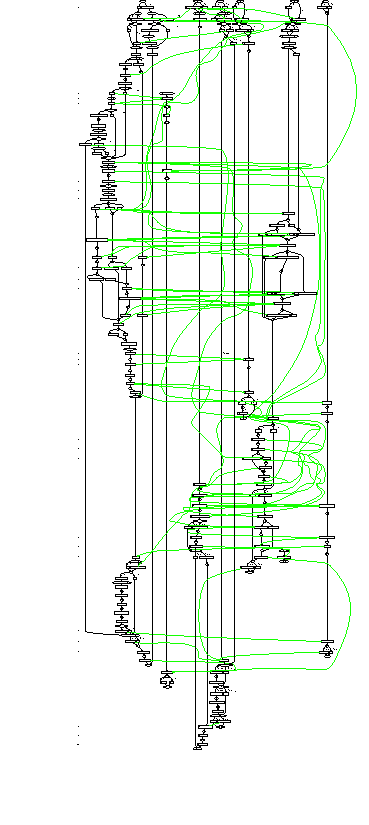
\includegraphics{stategraph.eps}}
\caption{Stategraph.}
\label{Figure: Stategraph}
\end{figure}
\end{document}
